\documentclass[a4paper,12pt]{scrartcl}
\usepackage[utf8x]{inputenc}
\usepackage[T1]{fontenc} % avec T1 comme option  d'encodage c'est ben mieux, surtout pour taper du français.
%\usepackage{lmodern,textcomp} % fortement conseillé pour les pdf. On peut mettre autre chose: kpfonts, fourier,...
\usepackage[french]{babel} %Sans ça les guillemets, amarchpo
\usepackage{amsmath}
\usepackage{multicol}
\usepackage{amssymb}
\usepackage{tkz-tab}
\usepackage{exercice_sheet}

%\trait
%\section*{}
%\exo{}
%\question{}
%\subquestion{}

\date{}

\renewcommand{\hasnotesprof}{0}


% Title Page
\title{Probabilités, généralités}

\author{\textsc{Mathématiques}}

\begin{document}

\maketitle

\tableofcontents

\section*{Introduction}

La \emph{théorie des probabilités} étudie les phénomènes aléatoires, c'est-à-dire les phénomènes régis par le hasard. Autrement dit, des expériences dont le résultat ne peut être prédit.

Le but des probabilités est alors d'arriver à dégager des tendances sur les issues d'une expérience aléatoire. Par exemple on sait de façon intuitive que lorsqu'on lance un pièce, on a \og{}environ une chance sur deux\fg{} d'obtenir \emph{pile} et autant d'obtenir \emph{face}. Et ce sans pour autant pouvoir prédire quel va être le résultat du lancer.

\section{Notion de probabilité}

\subsection{Vocabulaire}

\begin{enumerate}
 \item On appelle \textbf{expérience aléatoire} toute expérience dont on ne peut prédire l'issue mais reproductible (au moins en théorie). Dans la suite de ce paragraphe de vocabulaire, nous utiliserons l'expérience aléatoire d'un lancer de dé simple en guise d'exemple.
 
 \item On appelle \textbf{événement élémentaire} tout événement qui ne peut être scindé en plusieurs sous événements. 
 
 Exemple: les événement \og{}obtenir 1\fg{} ou \og{}obtenir 4\fg{} sont des événements élémentaires. En revanche, l'événement $A$: \og{}obtenir un nombre pair\fg{} n'est pas un événement élémentaire, vu qu'il est constitué des événements 2, 4 et 6: $A = \{2;4;6\}$.
 
 \item \textbf{L'univers des possibles} ou \emph{espace fondamental}, souvent noté $\Omega$ est l'ensemble des événements élémentaires. Pour notre lancer de dé, $\Omega = \{1;2;3;4;5;6\}$.
 
 \item La \textbf{probabilité} d'un événement est un nombre réel faisant état de son degré de certitude. C'est un nombre réel compris entre 0 et 1. Soit $E$ un événement d'une expérience aléatoire. Sa probabilité est notée $P(E)$, parfois $\mathbb{P}(E)$. Quelle que soit l'expérience, $0 \leqslant P(E) \leqslant 1$.
\end{enumerate}


\subsection{Exemple pratique}

Effectuons trois études statistiques sur un lancer de pièces lancée un plus ou moins grand nombre de fois. $\Omega = \{P;F\}$ où $P$ est l'événement \emph{Pile} et $F$ est l'événement \emph{Face}.

\begin{multicols}{2}
\begin{tabular}{|l|l|l|}
\hline
\multicolumn{3}{|c|}{\textbf{Avec 10 lancers}}                  \\ \hline
              & \textbf{Effectif} & \textbf{Fréquence} \\ \hline
\textbf{Pile} & 7                 & 0,7                \\ \hline
\textbf{Face} & 3                 & 0,3                \\ \hline
\end{tabular}

\vspace{2mm}

\begin{tabular}{|l|l|l|}
\hline
\multicolumn{3}{|c|}{\textbf{Avec 1000 lancers}}                  \\ \hline
              & \textbf{Effectif} & \textbf{Fréquence} \\ \hline
\textbf{Pile} & 481               & 0,481              \\ \hline
\textbf{Face} & 519               & 0,519              \\ \hline
\end{tabular}

\vspace{2mm}

\begin{tabular}{|l|l|l|}
\hline
\multicolumn{3}{|c|}{\textbf{Avec 100000 lancers}}                  \\ \hline
              & \textbf{Effectif} & \textbf{Fréquence} \\ \hline
\textbf{Pile} & 4965               & 0,4985              \\ \hline
\textbf{Face} & 5015               & 0,5015              \\ \hline
\end{tabular}

\end{multicols}

On remarque alors que la fréquence (au sens statistique du terme) se rapproche de $0.5$, lorsque le nombre de lancers augmente. En fait les fréquences de l'événement \emph{Pile} et de l'événement \emph{Face} s'approchent respectivement de $P(P)$ et de $P(F)$.

Dans cet exemple, $P(F) = P(P) = \frac{1}{2}$.

\subsection{En résumé}

\begin{itemize}
 \item À chaque événement $A$ on associe sa probabilité $P(A)$;
 \item Pour tout\footnote{En effet, une probabilité négative ou supérieure à 1 n'aurait aucun sens.} événement $A$, $0 \leqslant P(A) \leqslant 1$;
 \item La probabilité d'un événement certain est 1;
 \item La probabilité d'un événement impossible est 0;
 \item La probabilité d'un événement est la somme des probabilités des événements élémentaires réalisant cet événement;
 \item L'ensemble des événements élémentaires est l'univers des possibles $\Omega$.
\end{itemize}

%%LaTeX with PSTricks extensions
%%Creator: inkscape 0.92.4
%%Please note this file requires PSTricks extensions
\psset{xunit=.5pt,yunit=.5pt,runit=.5pt}
\begin{pspicture}(610.81919753,357.8644712)
{
\newrgbcolor{curcolor}{0 0 0}
\pscustom[linestyle=none,fillstyle=solid,fillcolor=curcolor,opacity=0.03862664]
{
\newpath
\moveto(428.21252813,159.01682784)
\curveto(428.21252813,71.71610722)(374.58852324,0.94488998)(308.43996098,0.94488998)
\curveto(242.29139872,0.94488998)(188.66739383,71.71610722)(188.66739383,159.01682784)
\curveto(188.66739383,246.31754847)(242.29139872,317.0887657)(308.43996098,317.0887657)
\curveto(374.58852324,317.0887657)(428.21252813,246.31754847)(428.21252813,159.01682784)
\closepath
}
}
{
\newrgbcolor{curcolor}{0 0 0}
\pscustom[linewidth=1.88976378,linecolor=curcolor]
{
\newpath
\moveto(428.21252813,159.01682784)
\curveto(428.21252813,71.71610722)(374.58852324,0.94488998)(308.43996098,0.94488998)
\curveto(242.29139872,0.94488998)(188.66739383,71.71610722)(188.66739383,159.01682784)
\curveto(188.66739383,246.31754847)(242.29139872,317.0887657)(308.43996098,317.0887657)
\curveto(374.58852324,317.0887657)(428.21252813,246.31754847)(428.21252813,159.01682784)
\closepath
}
}
{
\newrgbcolor{curcolor}{0 0 0}
\pscustom[linewidth=2.29233407,linecolor=curcolor]
{
\newpath
\moveto(235.78441224,74.73916141)
\lineto(257.7464558,74.73916141)
}
}
{
\newrgbcolor{curcolor}{0 0 0}
\pscustom[linewidth=2.29233407,linecolor=curcolor]
{
\newpath
\moveto(246.76543288,85.72019809)
\lineto(246.76543288,63.75814766)
}
}
{
\newrgbcolor{curcolor}{0 0 0}
\pscustom[linewidth=2.29233411,linecolor=curcolor]
{
\newpath
\moveto(332.0240438,116.00866174)
\lineto(353.98608772,116.00866174)
}
}
{
\newrgbcolor{curcolor}{0 0 0}
\pscustom[linewidth=2.29233411,linecolor=curcolor]
{
\newpath
\moveto(343.00506461,126.98969859)
\lineto(343.00506461,105.0276478)
}
}
{
\newrgbcolor{curcolor}{0 0 0}
\pscustom[linewidth=2.29233411,linecolor=curcolor]
{
\newpath
\moveto(364.55659561,227.47605323)
\lineto(386.51863953,227.47605323)
}
}
{
\newrgbcolor{curcolor}{0 0 0}
\pscustom[linewidth=2.29233411,linecolor=curcolor]
{
\newpath
\moveto(375.53761642,238.45709009)
\lineto(375.53761642,216.4950393)
}
}
{
\newrgbcolor{curcolor}{0 0 0}
\pscustom[linewidth=2.29233411,linecolor=curcolor]
{
\newpath
\moveto(371.37883183,186.89997134)
\lineto(393.34087575,186.89997134)
}
}
{
\newrgbcolor{curcolor}{0 0 0}
\pscustom[linewidth=2.29233411,linecolor=curcolor]
{
\newpath
\moveto(382.35985265,197.8810082)
\lineto(382.35985265,175.91895741)
}
}
{
\newrgbcolor{curcolor}{0 0 0}
\pscustom[linewidth=2.29233411,linecolor=curcolor]
{
\newpath
\moveto(339.69409231,47.87422646)
\lineto(361.65613622,47.87422646)
}
}
{
\newrgbcolor{curcolor}{0 0 0}
\pscustom[linewidth=2.29233411,linecolor=curcolor]
{
\newpath
\moveto(350.67511312,58.85526332)
\lineto(350.67511312,36.89321253)
}
}
{
\newrgbcolor{curcolor}{0 0 0}
\pscustom[linewidth=2.29233411,linecolor=curcolor]
{
\newpath
\moveto(375.09342711,211.74851685)
\lineto(397.05547102,211.74851685)
}
}
{
\newrgbcolor{curcolor}{0 0 0}
\pscustom[linewidth=2.29233411,linecolor=curcolor]
{
\newpath
\moveto(386.07444792,222.72955371)
\lineto(386.07444792,200.76750292)
}
}
{
\newrgbcolor{curcolor}{0 0 0}
\pscustom[linewidth=2.29233411,linecolor=curcolor]
{
\newpath
\moveto(268.10180884,93.59779055)
\lineto(290.06385276,93.59779055)
}
}
{
\newrgbcolor{curcolor}{0 0 0}
\pscustom[linewidth=2.29233411,linecolor=curcolor]
{
\newpath
\moveto(279.08282965,104.57882741)
\lineto(279.08282965,82.61677662)
}
}
{
\newrgbcolor{curcolor}{0 0 0}
\pscustom[linewidth=2.29233411,linecolor=curcolor]
{
\newpath
\moveto(255.72792286,243.85749701)
\lineto(277.68996677,243.85749701)
}
}
{
\newrgbcolor{curcolor}{0 0 0}
\pscustom[linewidth=2.29233411,linecolor=curcolor]
{
\newpath
\moveto(266.70894367,254.83853387)
\lineto(266.70894367,232.87648308)
}
}
{
\newrgbcolor{curcolor}{0 0 0}
\pscustom[linewidth=2.29233411,linecolor=curcolor]
{
\newpath
\moveto(229.17996947,160.5489767)
\lineto(251.14201339,160.5489767)
}
}
{
\newrgbcolor{curcolor}{0 0 0}
\pscustom[linewidth=2.29233411,linecolor=curcolor]
{
\newpath
\moveto(240.16099028,171.53001355)
\lineto(240.16099028,149.56796276)
}
}
{
\newrgbcolor{curcolor}{0 0 0}
\pscustom[linewidth=2.29233411,linecolor=curcolor]
{
\newpath
\moveto(318.68499876,246.42762489)
\lineto(340.64704268,246.42762489)
}
}
{
\newrgbcolor{curcolor}{0 0 0}
\pscustom[linewidth=2.29233411,linecolor=curcolor]
{
\newpath
\moveto(329.66601957,257.40866174)
\lineto(329.66601957,235.44661095)
}
}
{
\newrgbcolor{curcolor}{0 0 0}
\pscustom[linewidth=2.29233411,linecolor=curcolor]
{
\newpath
\moveto(286.94464349,48.43879339)
\lineto(308.9066874,48.43879339)
}
}
{
\newrgbcolor{curcolor}{0 0 0}
\pscustom[linewidth=2.29233411,linecolor=curcolor]
{
\newpath
\moveto(297.9256643,59.41983025)
\lineto(297.9256643,37.45777945)
}
}
{
\newrgbcolor{curcolor}{0 0 0}
\pscustom[linewidth=2.29233411,linecolor=curcolor]
{
\newpath
\moveto(275.2034353,212.27588567)
\lineto(297.16547921,212.27588567)
}
}
{
\newrgbcolor{curcolor}{0 0 0}
\pscustom[linewidth=2.29233411,linecolor=curcolor]
{
\newpath
\moveto(286.18445611,223.25692253)
\lineto(286.18445611,201.29487174)
}
}
{
\newrgbcolor{curcolor}{0 0 0}
\pscustom[linewidth=2.29233411,linecolor=curcolor]
{
\newpath
\moveto(280.76782207,166.34885071)
\lineto(302.72986599,166.34885071)
}
}
{
\newrgbcolor{curcolor}{0 0 0}
\pscustom[linewidth=2.29233411,linecolor=curcolor]
{
\newpath
\moveto(291.74884288,177.32988757)
\lineto(291.74884288,155.36783678)
}
}
{
\newrgbcolor{curcolor}{0 0 0}
\pscustom[linewidth=2.29233411,linecolor=curcolor]
{
\newpath
\moveto(331.77318144,177.05865607)
\lineto(353.73522536,177.05865607)
}
}
{
\newrgbcolor{curcolor}{0 0 0}
\pscustom[linewidth=2.29233411,linecolor=curcolor]
{
\newpath
\moveto(342.75420225,188.03969292)
\lineto(342.75420225,166.07764213)
}
}
{
\newrgbcolor{curcolor}{0 0 0}
\pscustom[linewidth=0.99999995,linecolor=curcolor]
{
\newpath
\moveto(234.02019402,283.86058836)
\lineto(149.32818142,313.40430868)
}
}
{
\newrgbcolor{curcolor}{0 0 0}
\pscustom[linestyle=none,fillstyle=solid,fillcolor=curcolor]
{
\newpath
\moveto(64.58390975,351.05446971)
\lineto(64.58390975,354.38446971)
\curveto(63.56390975,355.22446971)(62.27390975,355.67446971)(59.75390975,355.97446971)
\lineto(59.75390975,357.86446971)
\lineto(58.73390975,357.86446971)
\lineto(58.73390975,355.97446971)
\curveto(56.84390975,355.76446971)(56.00390975,355.49446971)(55.01390975,354.71446971)
\curveto(53.99390975,353.90446971)(53.39390975,352.70446971)(53.39390975,351.41446971)
\curveto(53.39390975,350.00446971)(53.87390975,348.95446971)(55.07390975,347.84446971)
\curveto(55.94390975,347.00446971)(56.60390975,346.55446971)(58.73390975,345.35446971)
\lineto(58.73390975,336.89446971)
\curveto(55.91390975,336.92446971)(54.32390975,338.33446971)(53.60390975,341.48446971)
\lineto(53.15390975,341.48446971)
\lineto(53.15390975,337.58446971)
\curveto(54.95390975,336.47446971)(56.21390975,336.14446971)(58.73390975,336.05446971)
\lineto(58.73390975,333.44446971)
\lineto(59.75390975,333.44446971)
\lineto(59.75390975,336.05446971)
\curveto(61.97390975,336.41446971)(62.90390975,336.77446971)(63.98390975,337.64446971)
\curveto(64.97390975,338.48446971)(65.54390975,339.71446971)(65.54390975,341.15446971)
\curveto(65.54390975,342.23446971)(65.33390975,343.22446971)(64.94390975,343.85446971)
\curveto(64.16390975,345.08446971)(63.35390975,345.71446971)(59.75390975,347.78446971)
\lineto(59.75390975,355.16446971)
\curveto(62.27390975,354.86446971)(63.62390975,353.60446971)(64.13390975,351.05446971)
\closepath
\moveto(58.70390975,348.26446971)
\curveto(56.18390975,349.94446971)(55.61390975,350.66446971)(55.61390975,352.07446971)
\curveto(55.61390975,353.72446971)(56.63390975,354.74446971)(58.70390975,355.16446971)
\closepath
\moveto(59.75390975,344.84446971)
\curveto(62.54390975,343.10446971)(63.17390975,342.29446971)(63.17390975,340.43446971)
\curveto(63.17390975,338.45446971)(62.09390975,337.34446971)(59.75390975,336.89446971)
\closepath
}
}
{
\newrgbcolor{curcolor}{0 0 0}
\pscustom[linestyle=none,fillstyle=solid,fillcolor=curcolor]
{
\newpath
\moveto(66.56390975,356.33446971)
\lineto(73.40390975,335.63446971)
\lineto(75.44390975,335.63446971)
\lineto(68.57390975,356.33446971)
\closepath
}
}
{
\newrgbcolor{curcolor}{0 0 0}
\pscustom[linestyle=none,fillstyle=solid,fillcolor=curcolor]
{
\newpath
\moveto(86.8631285,356.33446971)
\curveto(81.1331285,356.33446971)(77.0531285,352.04446971)(77.0531285,345.98446971)
\curveto(77.0531285,343.16446971)(78.0131285,340.40446971)(79.6331285,338.69446971)
\curveto(81.3731285,336.80446971)(84.0431285,335.63446971)(86.6831285,335.63446971)
\curveto(92.5931285,335.63446971)(96.6731285,339.80446971)(96.6731285,345.86446971)
\curveto(96.6731285,348.83446971)(95.8031285,351.41446971)(94.1531285,353.18446971)
\curveto(92.2631285,355.25446971)(89.7431285,356.33446971)(86.8631285,356.33446971)
\closepath
\moveto(86.8631285,355.25446971)
\curveto(88.2431285,355.25446971)(89.6231285,354.71446971)(90.7031285,353.75446971)
\curveto(92.3231285,352.28446971)(93.2531285,349.46446971)(93.2531285,345.89446971)
\curveto(93.2531285,344.12446971)(92.8931285,342.05446971)(92.2631285,340.49446971)
\curveto(91.9931285,339.74446971)(91.4831285,338.99446971)(90.7931285,338.30446971)
\curveto(89.7431285,337.25446971)(88.3931285,336.71446971)(86.8031285,336.71446971)
\curveto(85.4231285,336.71446971)(84.0731285,337.25446971)(82.9931285,338.18446971)
\curveto(81.4631285,339.56446971)(80.4731285,342.59446971)(80.4731285,345.92446971)
\curveto(80.4731285,348.98446971)(81.3131285,351.89446971)(82.5731285,353.30446971)
\curveto(83.7431285,354.59446971)(85.2131285,355.25446971)(86.8631285,355.25446971)
\closepath
}
}
{
\newrgbcolor{curcolor}{0 0 0}
\pscustom[linestyle=none,fillstyle=solid,fillcolor=curcolor]
{
\newpath
\moveto(98.192816,336.05446971)
\lineto(104.852816,336.05446971)
\lineto(104.852816,336.50446971)
\curveto(103.322816,336.53446971)(102.842816,336.86446971)(102.812816,338.06446971)
\lineto(102.812816,346.52446971)
\curveto(102.812816,346.58446971)(103.052816,346.88446971)(103.262816,347.09446971)
\curveto(104.012816,347.78446971)(105.302816,348.29446971)(106.352816,348.29446971)
\curveto(107.672816,348.29446971)(108.332816,347.24446971)(108.332816,345.14446971)
\lineto(108.332816,338.63446971)
\curveto(108.272816,336.92446971)(107.972816,336.59446971)(106.292816,336.50446971)
\lineto(106.292816,336.05446971)
\lineto(113.012816,336.05446971)
\lineto(113.012816,336.50446971)
\curveto(111.332816,336.50446971)(110.912816,336.98446971)(110.852816,338.90446971)
\lineto(110.852816,346.46446971)
\curveto(111.752816,347.75446971)(112.712816,348.29446971)(114.122816,348.29446971)
\curveto(115.832816,348.29446971)(116.372816,347.48446971)(116.372816,344.99446971)
\lineto(116.372816,338.66446971)
\curveto(116.312816,336.89446971)(116.132816,336.68446971)(114.392816,336.50446971)
\lineto(114.392816,336.05446971)
\lineto(120.962816,336.05446971)
\lineto(120.962816,336.50446971)
\lineto(120.182816,336.56446971)
\curveto(119.222816,336.71446971)(118.892816,337.16446971)(118.892816,338.33446971)
\lineto(118.892816,344.51446971)
\curveto(118.892816,348.05446971)(117.722816,349.85446971)(115.412816,349.85446971)
\curveto(113.672816,349.85446971)(112.142816,349.07446971)(110.522816,347.33446971)
\curveto(109.982816,349.04446971)(108.962816,349.85446971)(107.342816,349.85446971)
\curveto(105.992816,349.85446971)(105.182816,349.46446971)(102.692816,347.54446971)
\lineto(102.692816,349.79446971)
\lineto(102.482816,349.85446971)
\curveto(100.892816,349.28446971)(99.872816,348.95446971)(98.282816,348.50446971)
\lineto(98.282816,347.99446971)
\curveto(98.642816,348.08446971)(98.912816,348.11446971)(99.242816,348.11446971)
\curveto(100.022816,348.11446971)(100.292816,347.63446971)(100.292816,346.19446971)
\lineto(100.292816,338.60446971)
\curveto(100.232816,336.92446971)(99.842816,336.50446971)(98.192816,336.50446971)
\closepath
}
}
{
\newrgbcolor{curcolor}{0 0 0}
\pscustom[linestyle=none,fillstyle=solid,fillcolor=curcolor]
{
\newpath
\moveto(133.2731285,340.97446971)
\curveto(131.8331285,338.69446971)(130.5431285,337.82446971)(128.6231285,337.82446971)
\curveto(126.9131285,337.82446971)(125.6231285,338.69446971)(124.7531285,340.40446971)
\curveto(124.2131285,341.54446971)(124.0031285,342.50446971)(123.9431285,344.36446971)
\lineto(133.1831285,344.36446971)
\curveto(132.9431285,346.31446971)(132.6431285,347.18446971)(131.8931285,348.14446971)
\curveto(130.9931285,349.22446971)(129.6131285,349.85446971)(128.0531285,349.85446971)
\curveto(126.5531285,349.85446971)(125.1431285,349.31446971)(124.0031285,348.29446971)
\curveto(122.5931285,347.06446971)(121.7831285,344.93446971)(121.7831285,342.47446971)
\curveto(121.7831285,338.33446971)(123.9431285,335.75446971)(127.3931285,335.75446971)
\curveto(130.2431285,335.75446971)(132.4931285,337.52446971)(133.7531285,340.76446971)
\closepath
\moveto(124.0031285,345.32446971)
\curveto(124.3331285,347.66446971)(125.3531285,348.77446971)(127.1831285,348.77446971)
\curveto(129.0131285,348.77446971)(129.7331285,347.93446971)(130.1231285,345.32446971)
\closepath
}
}
{
\newrgbcolor{curcolor}{0 0 0}
\pscustom[linestyle=none,fillstyle=solid,fillcolor=curcolor]
{
\newpath
\moveto(147.73078475,347.69446971)
\lineto(147.73078475,348.86446971)
\lineto(145.42078475,348.86446971)
\curveto(144.79078475,348.86446971)(144.37078475,348.95446971)(143.77078475,349.16446971)
\lineto(143.11078475,349.40446971)
\curveto(142.33078475,349.70446971)(141.49078475,349.85446971)(140.71078475,349.85446971)
\curveto(137.92078475,349.85446971)(135.70078475,347.72446971)(135.70078475,344.96446971)
\curveto(135.70078475,343.07446971)(136.48078475,341.93446971)(138.49078475,340.94446971)
\lineto(137.71078475,340.22446971)
\curveto(137.08078475,339.62446971)(136.72078475,339.29446971)(136.63078475,339.17446971)
\curveto(136.00078475,338.51446971)(135.82078475,338.18446971)(135.82078475,337.67446971)
\curveto(135.82078475,337.01446971)(136.15078475,336.68446971)(137.41078475,336.08446971)
\curveto(135.25078475,334.52446971)(134.47078475,333.53446971)(134.47078475,332.42446971)
\curveto(134.47078475,330.83446971)(136.78078475,329.51446971)(139.66078475,329.51446971)
\curveto(141.91078475,329.51446971)(144.25078475,330.29446971)(145.81078475,331.55446971)
\curveto(146.95078475,332.48446971)(147.46078475,333.44446971)(147.46078475,334.58446971)
\curveto(147.46078475,336.44446971)(146.05078475,337.67446971)(143.83078475,337.79446971)
\lineto(139.96078475,337.97446971)
\curveto(138.34078475,338.03446971)(137.62078475,338.30446971)(137.62078475,338.78446971)
\curveto(137.62078475,339.38446971)(138.61078475,340.43446971)(139.42078475,340.67446971)
\curveto(140.50078475,340.58446971)(141.07078475,340.52446971)(141.13078475,340.52446971)
\curveto(142.24078475,340.52446971)(143.44078475,340.97446971)(144.37078475,341.78446971)
\curveto(145.36078475,342.62446971)(145.81078475,343.67446971)(145.81078475,345.17446971)
\curveto(145.81078475,346.04446971)(145.66078475,346.73446971)(145.24078475,347.69446971)
\closepath
\moveto(138.04078475,335.99446971)
\curveto(139.06078475,335.78446971)(141.40078475,335.60446971)(142.93078475,335.60446971)
\curveto(145.63078475,335.60446971)(146.62078475,335.21446971)(146.62078475,334.13446971)
\curveto(146.62078475,332.39446971)(144.34078475,331.22446971)(140.95078475,331.22446971)
\curveto(138.28078475,331.22446971)(136.57078475,332.09446971)(136.57078475,333.41446971)
\curveto(136.57078475,334.10446971)(136.84078475,334.55446971)(138.04078475,335.99446971)
\closepath
\moveto(138.19078475,346.19446971)
\curveto(138.19078475,347.96446971)(139.03078475,349.01446971)(140.41078475,349.01446971)
\curveto(141.34078475,349.01446971)(142.12078475,348.50446971)(142.60078475,347.60446971)
\curveto(143.17078475,346.55446971)(143.50078475,345.20446971)(143.50078475,344.00446971)
\curveto(143.50078475,342.32446971)(142.66078475,341.27446971)(141.28078475,341.27446971)
\curveto(139.42078475,341.27446971)(138.19078475,343.22446971)(138.19078475,346.10446971)
\closepath
}
}
{
\newrgbcolor{curcolor}{0 0 0}
\pscustom[linestyle=none,fillstyle=solid,fillcolor=curcolor]
{
\newpath
\moveto(161.18765975,338.03446971)
\curveto(160.67765975,337.61446971)(160.31765975,337.46446971)(159.86765975,337.46446971)
\curveto(159.17765975,337.46446971)(158.96765975,337.88446971)(158.96765975,339.20446971)
\lineto(158.96765975,345.05446971)
\curveto(158.96765975,346.61446971)(158.81765975,347.48446971)(158.36765975,348.20446971)
\curveto(157.70765975,349.28446971)(156.41765975,349.85446971)(154.64765975,349.85446971)
\curveto(151.82765975,349.85446971)(149.60765975,348.38446971)(149.60765975,346.49446971)
\curveto(149.60765975,345.80446971)(150.17765975,345.20446971)(150.89765975,345.20446971)
\curveto(151.61765975,345.20446971)(152.24765975,345.80446971)(152.24765975,346.46446971)
\curveto(152.24765975,346.58446971)(152.21765975,346.73446971)(152.18765975,346.94446971)
\curveto(152.12765975,347.21446971)(152.09765975,347.45446971)(152.09765975,347.66446971)
\curveto(152.09765975,348.47446971)(153.05765975,349.13446971)(154.25765975,349.13446971)
\curveto(155.72765975,349.13446971)(156.53765975,348.26446971)(156.53765975,346.64446971)
\lineto(156.53765975,344.81446971)
\curveto(151.94765975,342.98446971)(151.40765975,342.71446971)(150.11765975,341.57446971)
\curveto(149.45765975,340.97446971)(149.03765975,339.95446971)(149.03765975,338.96446971)
\curveto(149.03765975,337.07446971)(150.35765975,335.75446971)(152.18765975,335.75446971)
\curveto(153.50765975,335.75446971)(154.73765975,336.38446971)(156.56765975,337.94446971)
\curveto(156.71765975,336.35446971)(157.25765975,335.75446971)(158.48765975,335.75446971)
\curveto(159.50765975,335.75446971)(160.13765975,336.11446971)(161.18765975,337.25446971)
\closepath
\moveto(156.53765975,339.74446971)
\curveto(156.53765975,338.84446971)(156.38765975,338.51446971)(155.75765975,338.15446971)
\curveto(155.00765975,337.73446971)(154.19765975,337.49446971)(153.56765975,337.49446971)
\curveto(152.51765975,337.49446971)(151.67765975,338.51446971)(151.67765975,339.80446971)
\lineto(151.67765975,339.92446971)
\curveto(151.70765975,341.72446971)(153.02765975,342.86446971)(156.53765975,344.09446971)
\closepath
}
}
{
\newrgbcolor{curcolor}{0 0 0}
\pscustom[linestyle=none,fillstyle=solid,fillcolor=curcolor]
{
\newpath
\moveto(173.978441,351.05446971)
\lineto(173.978441,354.38446971)
\curveto(172.958441,355.22446971)(171.668441,355.67446971)(169.148441,355.97446971)
\lineto(169.148441,357.86446971)
\lineto(168.128441,357.86446971)
\lineto(168.128441,355.97446971)
\curveto(166.238441,355.76446971)(165.398441,355.49446971)(164.408441,354.71446971)
\curveto(163.388441,353.90446971)(162.788441,352.70446971)(162.788441,351.41446971)
\curveto(162.788441,350.00446971)(163.268441,348.95446971)(164.468441,347.84446971)
\curveto(165.338441,347.00446971)(165.998441,346.55446971)(168.128441,345.35446971)
\lineto(168.128441,336.89446971)
\curveto(165.308441,336.92446971)(163.718441,338.33446971)(162.998441,341.48446971)
\lineto(162.548441,341.48446971)
\lineto(162.548441,337.58446971)
\curveto(164.348441,336.47446971)(165.608441,336.14446971)(168.128441,336.05446971)
\lineto(168.128441,333.44446971)
\lineto(169.148441,333.44446971)
\lineto(169.148441,336.05446971)
\curveto(171.368441,336.41446971)(172.298441,336.77446971)(173.378441,337.64446971)
\curveto(174.368441,338.48446971)(174.938441,339.71446971)(174.938441,341.15446971)
\curveto(174.938441,342.23446971)(174.728441,343.22446971)(174.338441,343.85446971)
\curveto(173.558441,345.08446971)(172.748441,345.71446971)(169.148441,347.78446971)
\lineto(169.148441,355.16446971)
\curveto(171.668441,354.86446971)(173.018441,353.60446971)(173.528441,351.05446971)
\closepath
\moveto(168.098441,348.26446971)
\curveto(165.578441,349.94446971)(165.008441,350.66446971)(165.008441,352.07446971)
\curveto(165.008441,353.72446971)(166.028441,354.74446971)(168.098441,355.16446971)
\closepath
\moveto(169.148441,344.84446971)
\curveto(171.938441,343.10446971)(172.568441,342.29446971)(172.568441,340.43446971)
\curveto(172.568441,338.45446971)(171.488441,337.34446971)(169.148441,336.89446971)
\closepath
}
}
{
\newrgbcolor{curcolor}{0 0 0}
\pscustom[linestyle=none,fillstyle=solid,fillcolor=curcolor]
{
\newpath
\moveto(17.54999866,213.10171081)
\lineto(16.70999866,213.10171081)
\curveto(15.26999866,209.92171081)(13.91999866,209.17171081)(9.62999866,209.14171081)
\lineto(8.81999866,209.14171081)
\curveto(5.69999866,209.23171081)(5.66999866,209.26171081)(5.66999866,210.43171081)
\lineto(5.66999866,217.84171081)
\lineto(10.28999866,217.84171081)
\curveto(12.80999866,217.78171081)(13.19999866,217.42171081)(13.58999866,214.96171081)
\lineto(14.27999866,214.96171081)
\lineto(14.27999866,221.92171081)
\lineto(13.58999866,221.92171081)
\curveto(13.22999866,219.49171081)(12.80999866,219.13171081)(10.28999866,219.07171081)
\lineto(5.66999866,219.07171081)
\lineto(5.66999866,225.73171081)
\curveto(5.69999866,226.63171081)(5.81999866,226.75171081)(6.65999866,226.75171081)
\lineto(10.70999866,226.75171081)
\curveto(14.18999866,226.69171081)(14.78999866,226.27171081)(15.26999866,223.60171081)
\lineto(16.01999866,223.60171081)
\lineto(15.92999866,227.89171081)
\lineto(-0.00000134,227.89171081)
\lineto(-0.00000134,227.32171081)
\curveto(2.18999866,227.17171081)(2.54999866,226.78171081)(2.60999866,224.62171081)
\lineto(2.60999866,211.30171081)
\curveto(2.54999866,209.14171081)(2.15999866,208.72171081)(-0.00000134,208.60171081)
\lineto(-0.00000134,208.03171081)
\lineto(16.19999866,208.03171081)
\closepath
\moveto(7.82999866,229.60171081)
\lineto(12.44999866,232.51171081)
\curveto(13.07999866,232.90171081)(13.34999866,233.29171081)(13.34999866,233.77171081)
\curveto(13.34999866,234.37171081)(12.95999866,234.73171081)(12.29999866,234.73171081)
\curveto(11.84999866,234.73171081)(11.57999866,234.58171081)(11.03999866,234.04171081)
\lineto(6.62999866,229.60171081)
\closepath
}
}
{
\newrgbcolor{curcolor}{0 0 0}
\pscustom[linestyle=none,fillstyle=solid,fillcolor=curcolor]
{
\newpath
\moveto(32.28984241,221.53171081)
\lineto(28.11984241,221.53171081)
\lineto(28.11984241,221.08171081)
\curveto(29.07984241,220.99171081)(29.52984241,220.69171081)(29.52984241,220.12171081)
\curveto(29.52984241,219.82171081)(29.46984241,219.52171081)(29.34984241,219.22171081)
\lineto(26.37984241,211.45171081)
\lineto(23.31984241,219.13171081)
\curveto(23.13984241,219.55171081)(23.04984241,219.97171081)(23.04984241,220.24171081)
\curveto(23.04984241,220.78171081)(23.37984241,220.99171081)(24.42984241,221.08171081)
\lineto(24.42984241,221.53171081)
\lineto(18.54984241,221.53171081)
\lineto(18.54984241,221.08171081)
\curveto(19.68984241,221.02171081)(19.89984241,220.72171081)(21.27984241,217.63171081)
\lineto(24.87984241,209.02171081)
\curveto(24.93984241,208.84171081)(25.02984241,208.63171081)(25.11984241,208.39171081)
\curveto(25.20984241,208.15171081)(25.29984241,207.94171081)(25.38984241,207.79171081)
\curveto(25.44984241,207.67171081)(25.56984241,207.61171081)(25.65984241,207.61171081)
\curveto(25.83984241,207.61171081)(26.04984241,208.00171081)(26.49984241,209.11171081)
\lineto(30.33984241,218.74171081)
\curveto(31.20984241,220.78171081)(31.38984241,220.99171081)(32.28984241,221.08171081)
\closepath
}
}
{
\newrgbcolor{curcolor}{0 0 0}
\pscustom[linestyle=none,fillstyle=solid,fillcolor=curcolor]
{
\newpath
\moveto(44.10656116,212.95171081)
\curveto(42.66656116,210.67171081)(41.37656116,209.80171081)(39.45656116,209.80171081)
\curveto(37.74656116,209.80171081)(36.45656116,210.67171081)(35.58656116,212.38171081)
\curveto(35.04656116,213.52171081)(34.83656116,214.48171081)(34.77656116,216.34171081)
\lineto(44.01656116,216.34171081)
\curveto(43.77656116,218.29171081)(43.47656116,219.16171081)(42.72656116,220.12171081)
\curveto(41.82656116,221.20171081)(40.44656116,221.83171081)(38.88656116,221.83171081)
\curveto(37.38656116,221.83171081)(35.97656116,221.29171081)(34.83656116,220.27171081)
\curveto(33.42656116,219.04171081)(32.61656116,216.91171081)(32.61656116,214.45171081)
\curveto(32.61656116,210.31171081)(34.77656116,207.73171081)(38.22656116,207.73171081)
\curveto(41.07656116,207.73171081)(43.32656116,209.50171081)(44.58656116,212.74171081)
\closepath
\moveto(34.83656116,217.30171081)
\curveto(35.16656116,219.64171081)(36.18656116,220.75171081)(38.01656116,220.75171081)
\curveto(39.84656116,220.75171081)(40.56656116,219.91171081)(40.95656116,217.30171081)
\closepath
\moveto(37.53656116,223.24171081)
\lineto(42.12656116,226.15171081)
\curveto(42.78656116,226.57171081)(43.05656116,226.93171081)(43.05656116,227.41171081)
\curveto(43.05656116,228.01171081)(42.66656116,228.37171081)(42.00656116,228.37171081)
\curveto(41.55656116,228.37171081)(41.28656116,228.22171081)(40.74656116,227.68171081)
\lineto(36.33656116,223.24171081)
\closepath
}
}
{
\newrgbcolor{curcolor}{0 0 0}
\pscustom[linestyle=none,fillstyle=solid,fillcolor=curcolor]
{
\newpath
\moveto(45.70734241,208.03171081)
\lineto(52.06734241,208.03171081)
\lineto(52.06734241,208.48171081)
\curveto(50.56734241,208.57171081)(50.08734241,208.96171081)(50.08734241,210.04171081)
\lineto(50.08734241,218.47171081)
\curveto(51.52734241,219.82171081)(52.18734241,220.18171081)(53.17734241,220.18171081)
\curveto(54.64734241,220.18171081)(55.36734241,219.25171081)(55.36734241,217.27171081)
\lineto(55.36734241,211.00171081)
\curveto(55.30734241,209.05171081)(54.94734241,208.57171081)(53.47734241,208.48171081)
\lineto(53.47734241,208.03171081)
\lineto(59.71734241,208.03171081)
\lineto(59.71734241,208.48171081)
\curveto(58.24734241,208.63171081)(57.91734241,208.99171081)(57.88734241,210.46171081)
\lineto(57.88734241,217.33171081)
\curveto(57.88734241,220.15171081)(56.56734241,221.83171081)(54.34734241,221.83171081)
\curveto(52.96734241,221.83171081)(52.03734241,221.32171081)(49.99734241,219.40171081)
\lineto(49.99734241,221.77171081)
\lineto(49.78734241,221.83171081)
\curveto(48.22734241,221.26171081)(47.20734241,220.93171081)(45.64734241,220.48171081)
\lineto(45.64734241,219.97171081)
\curveto(45.85734241,220.06171081)(46.12734241,220.09171081)(46.45734241,220.09171081)
\curveto(47.29734241,220.09171081)(47.56734241,219.64171081)(47.56734241,218.17171081)
\lineto(47.56734241,210.73171081)
\curveto(47.53734241,208.96171081)(47.20734241,208.57171081)(45.70734241,208.48171081)
\closepath
}
}
{
\newrgbcolor{curcolor}{0 0 0}
\pscustom[linestyle=none,fillstyle=solid,fillcolor=curcolor]
{
\newpath
\moveto(72.40734241,212.95171081)
\curveto(70.96734241,210.67171081)(69.67734241,209.80171081)(67.75734241,209.80171081)
\curveto(66.04734241,209.80171081)(64.75734241,210.67171081)(63.88734241,212.38171081)
\curveto(63.34734241,213.52171081)(63.13734241,214.48171081)(63.07734241,216.34171081)
\lineto(72.31734241,216.34171081)
\curveto(72.07734241,218.29171081)(71.77734241,219.16171081)(71.02734241,220.12171081)
\curveto(70.12734241,221.20171081)(68.74734241,221.83171081)(67.18734241,221.83171081)
\curveto(65.68734241,221.83171081)(64.27734241,221.29171081)(63.13734241,220.27171081)
\curveto(61.72734241,219.04171081)(60.91734241,216.91171081)(60.91734241,214.45171081)
\curveto(60.91734241,210.31171081)(63.07734241,207.73171081)(66.52734241,207.73171081)
\curveto(69.37734241,207.73171081)(71.62734241,209.50171081)(72.88734241,212.74171081)
\closepath
\moveto(63.13734241,217.30171081)
\curveto(63.46734241,219.64171081)(64.48734241,220.75171081)(66.31734241,220.75171081)
\curveto(68.14734241,220.75171081)(68.86734241,219.91171081)(69.25734241,217.30171081)
\closepath
}
}
{
\newrgbcolor{curcolor}{0 0 0}
\pscustom[linestyle=none,fillstyle=solid,fillcolor=curcolor]
{
\newpath
\moveto(73.94812366,208.03171081)
\lineto(80.60812366,208.03171081)
\lineto(80.60812366,208.48171081)
\curveto(79.07812366,208.51171081)(78.59812366,208.84171081)(78.56812366,210.04171081)
\lineto(78.56812366,218.50171081)
\curveto(78.56812366,218.56171081)(78.80812366,218.86171081)(79.01812366,219.07171081)
\curveto(79.76812366,219.76171081)(81.05812366,220.27171081)(82.10812366,220.27171081)
\curveto(83.42812366,220.27171081)(84.08812366,219.22171081)(84.08812366,217.12171081)
\lineto(84.08812366,210.61171081)
\curveto(84.02812366,208.90171081)(83.72812366,208.57171081)(82.04812366,208.48171081)
\lineto(82.04812366,208.03171081)
\lineto(88.76812366,208.03171081)
\lineto(88.76812366,208.48171081)
\curveto(87.08812366,208.48171081)(86.66812366,208.96171081)(86.60812366,210.88171081)
\lineto(86.60812366,218.44171081)
\curveto(87.50812366,219.73171081)(88.46812366,220.27171081)(89.87812366,220.27171081)
\curveto(91.58812366,220.27171081)(92.12812366,219.46171081)(92.12812366,216.97171081)
\lineto(92.12812366,210.64171081)
\curveto(92.06812366,208.87171081)(91.88812366,208.66171081)(90.14812366,208.48171081)
\lineto(90.14812366,208.03171081)
\lineto(96.71812366,208.03171081)
\lineto(96.71812366,208.48171081)
\lineto(95.93812366,208.54171081)
\curveto(94.97812366,208.69171081)(94.64812366,209.14171081)(94.64812366,210.31171081)
\lineto(94.64812366,216.49171081)
\curveto(94.64812366,220.03171081)(93.47812366,221.83171081)(91.16812366,221.83171081)
\curveto(89.42812366,221.83171081)(87.89812366,221.05171081)(86.27812366,219.31171081)
\curveto(85.73812366,221.02171081)(84.71812366,221.83171081)(83.09812366,221.83171081)
\curveto(81.74812366,221.83171081)(80.93812366,221.44171081)(78.44812366,219.52171081)
\lineto(78.44812366,221.77171081)
\lineto(78.23812366,221.83171081)
\curveto(76.64812366,221.26171081)(75.62812366,220.93171081)(74.03812366,220.48171081)
\lineto(74.03812366,219.97171081)
\curveto(74.39812366,220.06171081)(74.66812366,220.09171081)(74.99812366,220.09171081)
\curveto(75.77812366,220.09171081)(76.04812366,219.61171081)(76.04812366,218.17171081)
\lineto(76.04812366,210.58171081)
\curveto(75.98812366,208.90171081)(75.59812366,208.48171081)(73.94812366,208.48171081)
\closepath
}
}
{
\newrgbcolor{curcolor}{0 0 0}
\pscustom[linestyle=none,fillstyle=solid,fillcolor=curcolor]
{
\newpath
\moveto(109.02843616,212.95171081)
\curveto(107.58843616,210.67171081)(106.29843616,209.80171081)(104.37843616,209.80171081)
\curveto(102.66843616,209.80171081)(101.37843616,210.67171081)(100.50843616,212.38171081)
\curveto(99.96843616,213.52171081)(99.75843616,214.48171081)(99.69843616,216.34171081)
\lineto(108.93843616,216.34171081)
\curveto(108.69843616,218.29171081)(108.39843616,219.16171081)(107.64843616,220.12171081)
\curveto(106.74843616,221.20171081)(105.36843616,221.83171081)(103.80843616,221.83171081)
\curveto(102.30843616,221.83171081)(100.89843616,221.29171081)(99.75843616,220.27171081)
\curveto(98.34843616,219.04171081)(97.53843616,216.91171081)(97.53843616,214.45171081)
\curveto(97.53843616,210.31171081)(99.69843616,207.73171081)(103.14843616,207.73171081)
\curveto(105.99843616,207.73171081)(108.24843616,209.50171081)(109.50843616,212.74171081)
\closepath
\moveto(99.75843616,217.30171081)
\curveto(100.08843616,219.64171081)(101.10843616,220.75171081)(102.93843616,220.75171081)
\curveto(104.76843616,220.75171081)(105.48843616,219.91171081)(105.87843616,217.30171081)
\closepath
}
}
{
\newrgbcolor{curcolor}{0 0 0}
\pscustom[linestyle=none,fillstyle=solid,fillcolor=curcolor]
{
\newpath
\moveto(110.62921741,208.03171081)
\lineto(116.98921741,208.03171081)
\lineto(116.98921741,208.48171081)
\curveto(115.48921741,208.57171081)(115.00921741,208.96171081)(115.00921741,210.04171081)
\lineto(115.00921741,218.47171081)
\curveto(116.44921741,219.82171081)(117.10921741,220.18171081)(118.09921741,220.18171081)
\curveto(119.56921741,220.18171081)(120.28921741,219.25171081)(120.28921741,217.27171081)
\lineto(120.28921741,211.00171081)
\curveto(120.22921741,209.05171081)(119.86921741,208.57171081)(118.39921741,208.48171081)
\lineto(118.39921741,208.03171081)
\lineto(124.63921741,208.03171081)
\lineto(124.63921741,208.48171081)
\curveto(123.16921741,208.63171081)(122.83921741,208.99171081)(122.80921741,210.46171081)
\lineto(122.80921741,217.33171081)
\curveto(122.80921741,220.15171081)(121.48921741,221.83171081)(119.26921741,221.83171081)
\curveto(117.88921741,221.83171081)(116.95921741,221.32171081)(114.91921741,219.40171081)
\lineto(114.91921741,221.77171081)
\lineto(114.70921741,221.83171081)
\curveto(113.14921741,221.26171081)(112.12921741,220.93171081)(110.56921741,220.48171081)
\lineto(110.56921741,219.97171081)
\curveto(110.77921741,220.06171081)(111.04921741,220.09171081)(111.37921741,220.09171081)
\curveto(112.21921741,220.09171081)(112.48921741,219.64171081)(112.48921741,218.17171081)
\lineto(112.48921741,210.73171081)
\curveto(112.45921741,208.96171081)(112.12921741,208.57171081)(110.62921741,208.48171081)
\closepath
}
}
{
\newrgbcolor{curcolor}{0 0 0}
\pscustom[linestyle=none,fillstyle=solid,fillcolor=curcolor]
{
\newpath
\moveto(132.73921741,221.53171081)
\lineto(129.70921741,221.53171081)
\lineto(129.70921741,225.01171081)
\curveto(129.70921741,225.31171081)(129.64921741,225.40171081)(129.49921741,225.40171081)
\curveto(127.75921741,222.88171081)(126.85921741,221.86171081)(125.98921741,221.35171081)
\curveto(125.65921741,221.14171081)(125.47921741,220.96171081)(125.47921741,220.78171081)
\curveto(125.47921741,220.69171081)(125.50921741,220.63171081)(125.59921741,220.57171081)
\lineto(127.18921741,220.57171081)
\lineto(127.18921741,211.54171081)
\curveto(127.18921741,209.02171081)(128.08921741,207.73171081)(129.85921741,207.73171081)
\curveto(131.32921741,207.73171081)(132.46921741,208.45171081)(133.45921741,210.01171081)
\lineto(133.06921741,210.34171081)
\curveto(132.40921741,209.56171081)(131.92921741,209.29171081)(131.26921741,209.29171081)
\curveto(130.15921741,209.29171081)(129.70921741,210.10171081)(129.70921741,211.99171081)
\lineto(129.70921741,220.57171081)
\lineto(132.73921741,220.57171081)
\closepath
}
}
{
\newrgbcolor{curcolor}{0 0 0}
\pscustom[linestyle=none,fillstyle=solid,fillcolor=curcolor]
{
\newpath
\moveto(142.97671741,217.45171081)
\lineto(142.85671741,221.56171081)
\lineto(142.52671741,221.56171081)
\curveto(142.37671741,221.32171081)(142.22671741,221.23171081)(142.04671741,221.23171081)
\curveto(141.86671741,221.23171081)(141.56671741,221.29171081)(141.23671741,221.44171081)
\curveto(140.54671741,221.68171081)(139.85671741,221.83171081)(139.13671741,221.83171081)
\curveto(136.76671741,221.83171081)(135.05671741,220.27171081)(135.05671741,218.11171081)
\curveto(135.05671741,216.43171081)(136.01671741,215.23171081)(138.56671741,213.79171081)
\lineto(140.30671741,212.80171081)
\curveto(141.35671741,212.20171081)(141.86671741,211.48171081)(141.86671741,210.55171081)
\curveto(141.86671741,209.23171081)(140.90671741,208.39171081)(139.37671741,208.39171081)
\curveto(137.30671741,208.39171081)(136.25671741,209.53171081)(135.56671741,212.59171081)
\lineto(135.08671741,212.59171081)
\lineto(135.08671741,207.91171081)
\lineto(135.47671741,207.91171081)
\curveto(135.68671741,208.21171081)(135.80671741,208.27171081)(136.16671741,208.27171081)
\curveto(136.49671741,208.27171081)(136.85671741,208.21171081)(137.54671741,208.03171081)
\curveto(138.35671741,207.85171081)(139.13671741,207.73171081)(139.73671741,207.73171081)
\curveto(142.07671741,207.73171081)(143.96671741,209.47171081)(143.96671741,211.57171081)
\curveto(143.96671741,213.07171081)(143.24671741,214.06171081)(141.44671741,215.14171081)
\lineto(138.20671741,217.06171081)
\curveto(137.36671741,217.57171081)(136.91671741,218.29171081)(136.91671741,219.10171081)
\curveto(136.91671741,220.33171081)(137.84671741,221.14171081)(139.22671741,221.14171081)
\curveto(140.93671741,221.14171081)(141.83671741,220.15171081)(142.52671741,217.45171081)
\closepath
}
}
{
\newrgbcolor{curcolor}{0 0 0}
\pscustom[linestyle=none,fillstyle=solid,fillcolor=curcolor]
{
\newpath
\moveto(11.87999866,187.9517114)
\curveto(10.43999866,185.6717114)(9.14999866,184.8017114)(7.22999866,184.8017114)
\curveto(5.51999866,184.8017114)(4.22999866,185.6717114)(3.35999866,187.3817114)
\curveto(2.81999866,188.5217114)(2.60999866,189.4817114)(2.54999866,191.3417114)
\lineto(11.78999866,191.3417114)
\curveto(11.54999866,193.2917114)(11.24999866,194.1617114)(10.49999866,195.1217114)
\curveto(9.59999866,196.2017114)(8.21999866,196.8317114)(6.65999866,196.8317114)
\curveto(5.15999866,196.8317114)(3.74999866,196.2917114)(2.60999866,195.2717114)
\curveto(1.19999866,194.0417114)(0.38999866,191.9117114)(0.38999866,189.4517114)
\curveto(0.38999866,185.3117114)(2.54999866,182.7317114)(5.99999866,182.7317114)
\curveto(8.84999866,182.7317114)(11.09999866,184.5017114)(12.35999866,187.7417114)
\closepath
\moveto(2.60999866,192.3017114)
\curveto(2.93999866,194.6417114)(3.95999866,195.7517114)(5.78999866,195.7517114)
\curveto(7.61999866,195.7517114)(8.33999866,194.9117114)(8.72999866,192.3017114)
\closepath
\moveto(5.30999866,198.2417114)
\lineto(9.89999866,201.1517114)
\curveto(10.55999866,201.5717114)(10.82999866,201.9317114)(10.82999866,202.4117114)
\curveto(10.82999866,203.0117114)(10.43999866,203.3717114)(9.77999866,203.3717114)
\curveto(9.32999866,203.3717114)(9.05999866,203.2217114)(8.51999866,202.6817114)
\lineto(4.10999866,198.2417114)
\closepath
}
}
{
\newrgbcolor{curcolor}{0 0 0}
\pscustom[linestyle=none,fillstyle=solid,fillcolor=curcolor]
{
\newpath
\moveto(13.10202991,183.0317114)
\lineto(20.18202991,183.0317114)
\lineto(20.18202991,183.4817114)
\curveto(18.29202991,183.5717114)(17.96202991,183.8717114)(17.93202991,185.5517114)
\lineto(17.93202991,203.4617114)
\lineto(17.81202991,203.5217114)
\curveto(16.28202991,203.0417114)(15.17202991,202.7117114)(13.04202991,202.2017114)
\lineto(13.04202991,201.7217114)
\lineto(13.22202991,201.7217114)
\curveto(13.55202991,201.7517114)(13.91202991,201.7817114)(14.15202991,201.7817114)
\curveto(15.11202991,201.7817114)(15.41202991,201.3617114)(15.41202991,199.9517114)
\lineto(15.41202991,185.6417114)
\curveto(15.38202991,184.0217114)(14.96202991,183.6017114)(13.10202991,183.4817114)
\closepath
}
}
{
\newrgbcolor{curcolor}{0 0 0}
\pscustom[linestyle=none,fillstyle=solid,fillcolor=curcolor]
{
\newpath
\moveto(33.03234241,187.9517114)
\curveto(31.59234241,185.6717114)(30.30234241,184.8017114)(28.38234241,184.8017114)
\curveto(26.67234241,184.8017114)(25.38234241,185.6717114)(24.51234241,187.3817114)
\curveto(23.97234241,188.5217114)(23.76234241,189.4817114)(23.70234241,191.3417114)
\lineto(32.94234241,191.3417114)
\curveto(32.70234241,193.2917114)(32.40234241,194.1617114)(31.65234241,195.1217114)
\curveto(30.75234241,196.2017114)(29.37234241,196.8317114)(27.81234241,196.8317114)
\curveto(26.31234241,196.8317114)(24.90234241,196.2917114)(23.76234241,195.2717114)
\curveto(22.35234241,194.0417114)(21.54234241,191.9117114)(21.54234241,189.4517114)
\curveto(21.54234241,185.3117114)(23.70234241,182.7317114)(27.15234241,182.7317114)
\curveto(30.00234241,182.7317114)(32.25234241,184.5017114)(33.51234241,187.7417114)
\closepath
\moveto(23.76234241,192.3017114)
\curveto(24.09234241,194.6417114)(25.11234241,195.7517114)(26.94234241,195.7517114)
\curveto(28.77234241,195.7517114)(29.49234241,194.9117114)(29.88234241,192.3017114)
\closepath
\moveto(26.46234241,198.2417114)
\lineto(31.05234241,201.1517114)
\curveto(31.71234241,201.5717114)(31.98234241,201.9317114)(31.98234241,202.4117114)
\curveto(31.98234241,203.0117114)(31.59234241,203.3717114)(30.93234241,203.3717114)
\curveto(30.48234241,203.3717114)(30.21234241,203.2217114)(29.67234241,202.6817114)
\lineto(25.26234241,198.2417114)
\closepath
}
}
{
\newrgbcolor{curcolor}{0 0 0}
\pscustom[linestyle=none,fillstyle=solid,fillcolor=curcolor]
{
\newpath
\moveto(34.57312366,183.0317114)
\lineto(41.23312366,183.0317114)
\lineto(41.23312366,183.4817114)
\curveto(39.70312366,183.5117114)(39.22312366,183.8417114)(39.19312366,185.0417114)
\lineto(39.19312366,193.5017114)
\curveto(39.19312366,193.5617114)(39.43312366,193.8617114)(39.64312366,194.0717114)
\curveto(40.39312366,194.7617114)(41.68312366,195.2717114)(42.73312366,195.2717114)
\curveto(44.05312366,195.2717114)(44.71312366,194.2217114)(44.71312366,192.1217114)
\lineto(44.71312366,185.6117114)
\curveto(44.65312366,183.9017114)(44.35312366,183.5717114)(42.67312366,183.4817114)
\lineto(42.67312366,183.0317114)
\lineto(49.39312366,183.0317114)
\lineto(49.39312366,183.4817114)
\curveto(47.71312366,183.4817114)(47.29312366,183.9617114)(47.23312366,185.8817114)
\lineto(47.23312366,193.4417114)
\curveto(48.13312366,194.7317114)(49.09312366,195.2717114)(50.50312366,195.2717114)
\curveto(52.21312366,195.2717114)(52.75312366,194.4617114)(52.75312366,191.9717114)
\lineto(52.75312366,185.6417114)
\curveto(52.69312366,183.8717114)(52.51312366,183.6617114)(50.77312366,183.4817114)
\lineto(50.77312366,183.0317114)
\lineto(57.34312366,183.0317114)
\lineto(57.34312366,183.4817114)
\lineto(56.56312366,183.5417114)
\curveto(55.60312366,183.6917114)(55.27312366,184.1417114)(55.27312366,185.3117114)
\lineto(55.27312366,191.4917114)
\curveto(55.27312366,195.0317114)(54.10312366,196.8317114)(51.79312366,196.8317114)
\curveto(50.05312366,196.8317114)(48.52312366,196.0517114)(46.90312366,194.3117114)
\curveto(46.36312366,196.0217114)(45.34312366,196.8317114)(43.72312366,196.8317114)
\curveto(42.37312366,196.8317114)(41.56312366,196.4417114)(39.07312366,194.5217114)
\lineto(39.07312366,196.7717114)
\lineto(38.86312366,196.8317114)
\curveto(37.27312366,196.2617114)(36.25312366,195.9317114)(34.66312366,195.4817114)
\lineto(34.66312366,194.9717114)
\curveto(35.02312366,195.0617114)(35.29312366,195.0917114)(35.62312366,195.0917114)
\curveto(36.40312366,195.0917114)(36.67312366,194.6117114)(36.67312366,193.1717114)
\lineto(36.67312366,185.5817114)
\curveto(36.61312366,183.9017114)(36.22312366,183.4817114)(34.57312366,183.4817114)
\closepath
}
}
{
\newrgbcolor{curcolor}{0 0 0}
\pscustom[linestyle=none,fillstyle=solid,fillcolor=curcolor]
{
\newpath
\moveto(69.65343616,187.9517114)
\curveto(68.21343616,185.6717114)(66.92343616,184.8017114)(65.00343616,184.8017114)
\curveto(63.29343616,184.8017114)(62.00343616,185.6717114)(61.13343616,187.3817114)
\curveto(60.59343616,188.5217114)(60.38343616,189.4817114)(60.32343616,191.3417114)
\lineto(69.56343616,191.3417114)
\curveto(69.32343616,193.2917114)(69.02343616,194.1617114)(68.27343616,195.1217114)
\curveto(67.37343616,196.2017114)(65.99343616,196.8317114)(64.43343616,196.8317114)
\curveto(62.93343616,196.8317114)(61.52343616,196.2917114)(60.38343616,195.2717114)
\curveto(58.97343616,194.0417114)(58.16343616,191.9117114)(58.16343616,189.4517114)
\curveto(58.16343616,185.3117114)(60.32343616,182.7317114)(63.77343616,182.7317114)
\curveto(66.62343616,182.7317114)(68.87343616,184.5017114)(70.13343616,187.7417114)
\closepath
\moveto(60.38343616,192.3017114)
\curveto(60.71343616,194.6417114)(61.73343616,195.7517114)(63.56343616,195.7517114)
\curveto(65.39343616,195.7517114)(66.11343616,194.9117114)(66.50343616,192.3017114)
\closepath
}
}
{
\newrgbcolor{curcolor}{0 0 0}
\pscustom[linestyle=none,fillstyle=solid,fillcolor=curcolor]
{
\newpath
\moveto(71.25421741,183.0317114)
\lineto(77.61421741,183.0317114)
\lineto(77.61421741,183.4817114)
\curveto(76.11421741,183.5717114)(75.63421741,183.9617114)(75.63421741,185.0417114)
\lineto(75.63421741,193.4717114)
\curveto(77.07421741,194.8217114)(77.73421741,195.1817114)(78.72421741,195.1817114)
\curveto(80.19421741,195.1817114)(80.91421741,194.2517114)(80.91421741,192.2717114)
\lineto(80.91421741,186.0017114)
\curveto(80.85421741,184.0517114)(80.49421741,183.5717114)(79.02421741,183.4817114)
\lineto(79.02421741,183.0317114)
\lineto(85.26421741,183.0317114)
\lineto(85.26421741,183.4817114)
\curveto(83.79421741,183.6317114)(83.46421741,183.9917114)(83.43421741,185.4617114)
\lineto(83.43421741,192.3317114)
\curveto(83.43421741,195.1517114)(82.11421741,196.8317114)(79.89421741,196.8317114)
\curveto(78.51421741,196.8317114)(77.58421741,196.3217114)(75.54421741,194.4017114)
\lineto(75.54421741,196.7717114)
\lineto(75.33421741,196.8317114)
\curveto(73.77421741,196.2617114)(72.75421741,195.9317114)(71.19421741,195.4817114)
\lineto(71.19421741,194.9717114)
\curveto(71.40421741,195.0617114)(71.67421741,195.0917114)(72.00421741,195.0917114)
\curveto(72.84421741,195.0917114)(73.11421741,194.6417114)(73.11421741,193.1717114)
\lineto(73.11421741,185.7317114)
\curveto(73.08421741,183.9617114)(72.75421741,183.5717114)(71.25421741,183.4817114)
\closepath
}
}
{
\newrgbcolor{curcolor}{0 0 0}
\pscustom[linestyle=none,fillstyle=solid,fillcolor=curcolor]
{
\newpath
\moveto(93.36421741,196.5317114)
\lineto(90.33421741,196.5317114)
\lineto(90.33421741,200.0117114)
\curveto(90.33421741,200.3117114)(90.27421741,200.4017114)(90.12421741,200.4017114)
\curveto(88.38421741,197.8817114)(87.48421741,196.8617114)(86.61421741,196.3517114)
\curveto(86.28421741,196.1417114)(86.10421741,195.9617114)(86.10421741,195.7817114)
\curveto(86.10421741,195.6917114)(86.13421741,195.6317114)(86.22421741,195.5717114)
\lineto(87.81421741,195.5717114)
\lineto(87.81421741,186.5417114)
\curveto(87.81421741,184.0217114)(88.71421741,182.7317114)(90.48421741,182.7317114)
\curveto(91.95421741,182.7317114)(93.09421741,183.4517114)(94.08421741,185.0117114)
\lineto(93.69421741,185.3417114)
\curveto(93.03421741,184.5617114)(92.55421741,184.2917114)(91.89421741,184.2917114)
\curveto(90.78421741,184.2917114)(90.33421741,185.1017114)(90.33421741,186.9917114)
\lineto(90.33421741,195.5717114)
\lineto(93.36421741,195.5717114)
\closepath
}
}
{
\newrgbcolor{curcolor}{0 0 0}
\pscustom[linestyle=none,fillstyle=solid,fillcolor=curcolor]
{
\newpath
\moveto(107.58749866,185.0117114)
\curveto(107.07749866,184.5917114)(106.71749866,184.4417114)(106.26749866,184.4417114)
\curveto(105.57749866,184.4417114)(105.36749866,184.8617114)(105.36749866,186.1817114)
\lineto(105.36749866,192.0317114)
\curveto(105.36749866,193.5917114)(105.21749866,194.4617114)(104.76749866,195.1817114)
\curveto(104.10749866,196.2617114)(102.81749866,196.8317114)(101.04749866,196.8317114)
\curveto(98.22749866,196.8317114)(96.00749866,195.3617114)(96.00749866,193.4717114)
\curveto(96.00749866,192.7817114)(96.57749866,192.1817114)(97.29749866,192.1817114)
\curveto(98.01749866,192.1817114)(98.64749866,192.7817114)(98.64749866,193.4417114)
\curveto(98.64749866,193.5617114)(98.61749866,193.7117114)(98.58749866,193.9217114)
\curveto(98.52749866,194.1917114)(98.49749866,194.4317114)(98.49749866,194.6417114)
\curveto(98.49749866,195.4517114)(99.45749866,196.1117114)(100.65749866,196.1117114)
\curveto(102.12749866,196.1117114)(102.93749866,195.2417114)(102.93749866,193.6217114)
\lineto(102.93749866,191.7917114)
\curveto(98.34749866,189.9617114)(97.80749866,189.6917114)(96.51749866,188.5517114)
\curveto(95.85749866,187.9517114)(95.43749866,186.9317114)(95.43749866,185.9417114)
\curveto(95.43749866,184.0517114)(96.75749866,182.7317114)(98.58749866,182.7317114)
\curveto(99.90749866,182.7317114)(101.13749866,183.3617114)(102.96749866,184.9217114)
\curveto(103.11749866,183.3317114)(103.65749866,182.7317114)(104.88749866,182.7317114)
\curveto(105.90749866,182.7317114)(106.53749866,183.0917114)(107.58749866,184.2317114)
\closepath
\moveto(102.93749866,186.7217114)
\curveto(102.93749866,185.8217114)(102.78749866,185.4917114)(102.15749866,185.1317114)
\curveto(101.40749866,184.7117114)(100.59749866,184.4717114)(99.96749866,184.4717114)
\curveto(98.91749866,184.4717114)(98.07749866,185.4917114)(98.07749866,186.7817114)
\lineto(98.07749866,186.9017114)
\curveto(98.10749866,188.7017114)(99.42749866,189.8417114)(102.93749866,191.0717114)
\closepath
}
}
{
\newrgbcolor{curcolor}{0 0 0}
\pscustom[linestyle=none,fillstyle=solid,fillcolor=curcolor]
{
\newpath
\moveto(108.10827991,183.0317114)
\lineto(115.21827991,183.0317114)
\lineto(115.21827991,183.4817114)
\curveto(113.23827991,183.6317114)(113.02827991,183.9017114)(112.99827991,186.0917114)
\lineto(112.99827991,196.7417114)
\lineto(112.87827991,196.8317114)
\lineto(108.22827991,195.1817114)
\lineto(108.22827991,194.7317114)
\lineto(108.46827991,194.7617114)
\curveto(108.82827991,194.8217114)(109.18827991,194.8517114)(109.48827991,194.8517114)
\curveto(110.20827991,194.8517114)(110.47827991,194.3717114)(110.47827991,193.0517114)
\lineto(110.47827991,186.0917114)
\curveto(110.41827991,183.8717114)(110.14827991,183.5717114)(108.10827991,183.4817114)
\closepath
\moveto(111.46827991,203.5217114)
\curveto(110.65827991,203.5217114)(109.96827991,202.8317114)(109.96827991,201.9917114)
\curveto(109.96827991,201.1217114)(110.62827991,200.4617114)(111.46827991,200.4617114)
\curveto(112.36827991,200.4617114)(113.02827991,201.1217114)(113.02827991,201.9917114)
\curveto(113.02827991,202.8617114)(112.33827991,203.5217114)(111.46827991,203.5217114)
\closepath
}
}
{
\newrgbcolor{curcolor}{0 0 0}
\pscustom[linestyle=none,fillstyle=solid,fillcolor=curcolor]
{
\newpath
\moveto(116.09859241,183.0317114)
\lineto(123.29859241,183.0317114)
\lineto(123.29859241,183.4817114)
\curveto(121.28859241,183.5417114)(120.80859241,183.9617114)(120.74859241,185.7317114)
\lineto(120.74859241,192.4817114)
\curveto(120.74859241,193.4417114)(122.00859241,194.9417114)(122.84859241,194.9417114)
\curveto(123.02859241,194.9417114)(123.29859241,194.7917114)(123.62859241,194.4917114)
\curveto(124.07859241,194.0417114)(124.43859241,193.8917114)(124.82859241,193.8917114)
\curveto(125.54859241,193.8917114)(125.99859241,194.4017114)(125.99859241,195.2417114)
\curveto(125.99859241,196.2317114)(125.36859241,196.8317114)(124.34859241,196.8317114)
\curveto(123.08859241,196.8317114)(122.24859241,196.1717114)(120.74859241,194.0117114)
\lineto(120.74859241,196.7717114)
\lineto(120.59859241,196.8317114)
\curveto(118.91859241,196.1717114)(117.83859241,195.7517114)(116.15859241,195.2117114)
\lineto(116.15859241,194.7317114)
\curveto(116.57859241,194.8217114)(116.84859241,194.8517114)(117.20859241,194.8517114)
\curveto(117.95859241,194.8517114)(118.22859241,194.3717114)(118.22859241,193.0517114)
\lineto(118.22859241,185.5517114)
\curveto(118.16859241,183.9917114)(117.98859241,183.8117114)(116.09859241,183.4817114)
\closepath
}
}
{
\newrgbcolor{curcolor}{0 0 0}
\pscustom[linestyle=none,fillstyle=solid,fillcolor=curcolor]
{
\newpath
\moveto(138.03234241,187.9517114)
\curveto(136.59234241,185.6717114)(135.30234241,184.8017114)(133.38234241,184.8017114)
\curveto(131.67234241,184.8017114)(130.38234241,185.6717114)(129.51234241,187.3817114)
\curveto(128.97234241,188.5217114)(128.76234241,189.4817114)(128.70234241,191.3417114)
\lineto(137.94234241,191.3417114)
\curveto(137.70234241,193.2917114)(137.40234241,194.1617114)(136.65234241,195.1217114)
\curveto(135.75234241,196.2017114)(134.37234241,196.8317114)(132.81234241,196.8317114)
\curveto(131.31234241,196.8317114)(129.90234241,196.2917114)(128.76234241,195.2717114)
\curveto(127.35234241,194.0417114)(126.54234241,191.9117114)(126.54234241,189.4517114)
\curveto(126.54234241,185.3117114)(128.70234241,182.7317114)(132.15234241,182.7317114)
\curveto(135.00234241,182.7317114)(137.25234241,184.5017114)(138.51234241,187.7417114)
\closepath
\moveto(128.76234241,192.3017114)
\curveto(129.09234241,194.6417114)(130.11234241,195.7517114)(131.94234241,195.7517114)
\curveto(133.77234241,195.7517114)(134.49234241,194.9117114)(134.88234241,192.3017114)
\closepath
}
}
{
\newrgbcolor{curcolor}{0 0 0}
\pscustom[linestyle=none,fillstyle=solid,fillcolor=curcolor]
{
\newpath
\moveto(148.30874866,192.4517114)
\lineto(148.18874866,196.5617114)
\lineto(147.85874866,196.5617114)
\curveto(147.70874866,196.3217114)(147.55874866,196.2317114)(147.37874866,196.2317114)
\curveto(147.19874866,196.2317114)(146.89874866,196.2917114)(146.56874866,196.4417114)
\curveto(145.87874866,196.6817114)(145.18874866,196.8317114)(144.46874866,196.8317114)
\curveto(142.09874866,196.8317114)(140.38874866,195.2717114)(140.38874866,193.1117114)
\curveto(140.38874866,191.4317114)(141.34874866,190.2317114)(143.89874866,188.7917114)
\lineto(145.63874866,187.8017114)
\curveto(146.68874866,187.2017114)(147.19874866,186.4817114)(147.19874866,185.5517114)
\curveto(147.19874866,184.2317114)(146.23874866,183.3917114)(144.70874866,183.3917114)
\curveto(142.63874866,183.3917114)(141.58874866,184.5317114)(140.89874866,187.5917114)
\lineto(140.41874866,187.5917114)
\lineto(140.41874866,182.9117114)
\lineto(140.80874866,182.9117114)
\curveto(141.01874866,183.2117114)(141.13874866,183.2717114)(141.49874866,183.2717114)
\curveto(141.82874866,183.2717114)(142.18874866,183.2117114)(142.87874866,183.0317114)
\curveto(143.68874866,182.8517114)(144.46874866,182.7317114)(145.06874866,182.7317114)
\curveto(147.40874866,182.7317114)(149.29874866,184.4717114)(149.29874866,186.5717114)
\curveto(149.29874866,188.0717114)(148.57874866,189.0617114)(146.77874866,190.1417114)
\lineto(143.53874866,192.0617114)
\curveto(142.69874866,192.5717114)(142.24874866,193.2917114)(142.24874866,194.1017114)
\curveto(142.24874866,195.3317114)(143.17874866,196.1417114)(144.55874866,196.1417114)
\curveto(146.26874866,196.1417114)(147.16874866,195.1517114)(147.85874866,192.4517114)
\closepath
}
}
{
\newrgbcolor{curcolor}{0 0 0}
\pscustom[linewidth=0.99999995,linecolor=curcolor]
{
\newpath
\moveto(259.61058142,239.23435718)
\lineto(155.4689726,201.07369576)
}
}
{
\newrgbcolor{curcolor}{0 0 0}
\pscustom[linewidth=0.99999995,linecolor=curcolor]
{
\newpath
\moveto(279.44365228,171.22517923)
\lineto(155.4689726,201.07369576)
}
}
{
\newrgbcolor{curcolor}{0 0 0}
\pscustom[linewidth=0.99999995,linecolor=curcolor]
{
\newpath
\moveto(273.35732787,97.82894616)
\lineto(155.4689726,201.07369576)
}
}
{
\newrgbcolor{curcolor}{0 0 0}
\pscustom[linewidth=0.99999995,linecolor=curcolor]
{
\newpath
\moveto(233.6307137,164.53386584)
\lineto(155.4689726,201.07369576)
}
}
{
\newrgbcolor{curcolor}{0 0 0}
\pscustom[linewidth=1.88976378,linecolor=curcolor]
{
\newpath
\moveto(409.41102611,209.15416175)
\curveto(409.41102611,186.84824321)(396.94032908,168.76572344)(381.55694471,168.76572344)
\curveto(366.17356034,168.76572344)(353.70286331,186.84824321)(353.70286331,209.15416175)
\curveto(353.70286331,231.46008029)(366.17356034,249.54260006)(381.55694471,249.54260006)
\curveto(396.94032908,249.54260006)(409.41102611,231.46008029)(409.41102611,209.15416175)
\closepath
}
}
{
\newrgbcolor{curcolor}{0 0 0}
\pscustom[linestyle=none,fillstyle=solid,fillcolor=curcolor]
{
\newpath
\moveto(437.07000281,251.13081352)
\lineto(436.23000281,251.13081352)
\curveto(434.79000281,247.95081352)(433.44000281,247.20081352)(429.15000281,247.17081352)
\lineto(428.34000281,247.17081352)
\curveto(425.22000281,247.26081352)(425.19000281,247.29081352)(425.19000281,248.46081352)
\lineto(425.19000281,255.87081352)
\lineto(429.81000281,255.87081352)
\curveto(432.33000281,255.81081352)(432.72000281,255.45081352)(433.11000281,252.99081352)
\lineto(433.80000281,252.99081352)
\lineto(433.80000281,259.95081352)
\lineto(433.11000281,259.95081352)
\curveto(432.75000281,257.52081352)(432.33000281,257.16081352)(429.81000281,257.10081352)
\lineto(425.19000281,257.10081352)
\lineto(425.19000281,263.76081352)
\curveto(425.22000281,264.66081352)(425.34000281,264.78081352)(426.18000281,264.78081352)
\lineto(430.23000281,264.78081352)
\curveto(433.71000281,264.72081352)(434.31000281,264.30081352)(434.79000281,261.63081352)
\lineto(435.54000281,261.63081352)
\lineto(435.45000281,265.92081352)
\lineto(419.52000281,265.92081352)
\lineto(419.52000281,265.35081352)
\curveto(421.71000281,265.20081352)(422.07000281,264.81081352)(422.13000281,262.65081352)
\lineto(422.13000281,249.33081352)
\curveto(422.07000281,247.17081352)(421.68000281,246.75081352)(419.52000281,246.63081352)
\lineto(419.52000281,246.06081352)
\lineto(435.72000281,246.06081352)
\closepath
\moveto(427.35000281,267.63081352)
\lineto(431.97000281,270.54081352)
\curveto(432.60000281,270.93081352)(432.87000281,271.32081352)(432.87000281,271.80081352)
\curveto(432.87000281,272.40081352)(432.48000281,272.76081352)(431.82000281,272.76081352)
\curveto(431.37000281,272.76081352)(431.10000281,272.61081352)(430.56000281,272.07081352)
\lineto(426.15000281,267.63081352)
\closepath
}
}
{
\newrgbcolor{curcolor}{0 0 0}
\pscustom[linestyle=none,fillstyle=solid,fillcolor=curcolor]
{
\newpath
\moveto(451.80984656,259.56081352)
\lineto(447.63984656,259.56081352)
\lineto(447.63984656,259.11081352)
\curveto(448.59984656,259.02081352)(449.04984656,258.72081352)(449.04984656,258.15081352)
\curveto(449.04984656,257.85081352)(448.98984656,257.55081352)(448.86984656,257.25081352)
\lineto(445.89984656,249.48081352)
\lineto(442.83984656,257.16081352)
\curveto(442.65984656,257.58081352)(442.56984656,258.00081352)(442.56984656,258.27081352)
\curveto(442.56984656,258.81081352)(442.89984656,259.02081352)(443.94984656,259.11081352)
\lineto(443.94984656,259.56081352)
\lineto(438.06984656,259.56081352)
\lineto(438.06984656,259.11081352)
\curveto(439.20984656,259.05081352)(439.41984656,258.75081352)(440.79984656,255.66081352)
\lineto(444.39984656,247.05081352)
\curveto(444.45984656,246.87081352)(444.54984656,246.66081352)(444.63984656,246.42081352)
\curveto(444.72984656,246.18081352)(444.81984656,245.97081352)(444.90984656,245.82081352)
\curveto(444.96984656,245.70081352)(445.08984656,245.64081352)(445.17984656,245.64081352)
\curveto(445.35984656,245.64081352)(445.56984656,246.03081352)(446.01984656,247.14081352)
\lineto(449.85984656,256.77081352)
\curveto(450.72984656,258.81081352)(450.90984656,259.02081352)(451.80984656,259.11081352)
\closepath
}
}
{
\newrgbcolor{curcolor}{0 0 0}
\pscustom[linestyle=none,fillstyle=solid,fillcolor=curcolor]
{
\newpath
\moveto(463.62656531,250.98081352)
\curveto(462.18656531,248.70081352)(460.89656531,247.83081352)(458.97656531,247.83081352)
\curveto(457.26656531,247.83081352)(455.97656531,248.70081352)(455.10656531,250.41081352)
\curveto(454.56656531,251.55081352)(454.35656531,252.51081352)(454.29656531,254.37081352)
\lineto(463.53656531,254.37081352)
\curveto(463.29656531,256.32081352)(462.99656531,257.19081352)(462.24656531,258.15081352)
\curveto(461.34656531,259.23081352)(459.96656531,259.86081352)(458.40656531,259.86081352)
\curveto(456.90656531,259.86081352)(455.49656531,259.32081352)(454.35656531,258.30081352)
\curveto(452.94656531,257.07081352)(452.13656531,254.94081352)(452.13656531,252.48081352)
\curveto(452.13656531,248.34081352)(454.29656531,245.76081352)(457.74656531,245.76081352)
\curveto(460.59656531,245.76081352)(462.84656531,247.53081352)(464.10656531,250.77081352)
\closepath
\moveto(454.35656531,255.33081352)
\curveto(454.68656531,257.67081352)(455.70656531,258.78081352)(457.53656531,258.78081352)
\curveto(459.36656531,258.78081352)(460.08656531,257.94081352)(460.47656531,255.33081352)
\closepath
\moveto(457.05656531,261.27081352)
\lineto(461.64656531,264.18081352)
\curveto(462.30656531,264.60081352)(462.57656531,264.96081352)(462.57656531,265.44081352)
\curveto(462.57656531,266.04081352)(462.18656531,266.40081352)(461.52656531,266.40081352)
\curveto(461.07656531,266.40081352)(460.80656531,266.25081352)(460.26656531,265.71081352)
\lineto(455.85656531,261.27081352)
\closepath
}
}
{
\newrgbcolor{curcolor}{0 0 0}
\pscustom[linestyle=none,fillstyle=solid,fillcolor=curcolor]
{
\newpath
\moveto(465.22734656,246.06081352)
\lineto(471.58734656,246.06081352)
\lineto(471.58734656,246.51081352)
\curveto(470.08734656,246.60081352)(469.60734656,246.99081352)(469.60734656,248.07081352)
\lineto(469.60734656,256.50081352)
\curveto(471.04734656,257.85081352)(471.70734656,258.21081352)(472.69734656,258.21081352)
\curveto(474.16734656,258.21081352)(474.88734656,257.28081352)(474.88734656,255.30081352)
\lineto(474.88734656,249.03081352)
\curveto(474.82734656,247.08081352)(474.46734656,246.60081352)(472.99734656,246.51081352)
\lineto(472.99734656,246.06081352)
\lineto(479.23734656,246.06081352)
\lineto(479.23734656,246.51081352)
\curveto(477.76734656,246.66081352)(477.43734656,247.02081352)(477.40734656,248.49081352)
\lineto(477.40734656,255.36081352)
\curveto(477.40734656,258.18081352)(476.08734656,259.86081352)(473.86734656,259.86081352)
\curveto(472.48734656,259.86081352)(471.55734656,259.35081352)(469.51734656,257.43081352)
\lineto(469.51734656,259.80081352)
\lineto(469.30734656,259.86081352)
\curveto(467.74734656,259.29081352)(466.72734656,258.96081352)(465.16734656,258.51081352)
\lineto(465.16734656,258.00081352)
\curveto(465.37734656,258.09081352)(465.64734656,258.12081352)(465.97734656,258.12081352)
\curveto(466.81734656,258.12081352)(467.08734656,257.67081352)(467.08734656,256.20081352)
\lineto(467.08734656,248.76081352)
\curveto(467.05734656,246.99081352)(466.72734656,246.60081352)(465.22734656,246.51081352)
\closepath
}
}
{
\newrgbcolor{curcolor}{0 0 0}
\pscustom[linestyle=none,fillstyle=solid,fillcolor=curcolor]
{
\newpath
\moveto(491.92734656,250.98081352)
\curveto(490.48734656,248.70081352)(489.19734656,247.83081352)(487.27734656,247.83081352)
\curveto(485.56734656,247.83081352)(484.27734656,248.70081352)(483.40734656,250.41081352)
\curveto(482.86734656,251.55081352)(482.65734656,252.51081352)(482.59734656,254.37081352)
\lineto(491.83734656,254.37081352)
\curveto(491.59734656,256.32081352)(491.29734656,257.19081352)(490.54734656,258.15081352)
\curveto(489.64734656,259.23081352)(488.26734656,259.86081352)(486.70734656,259.86081352)
\curveto(485.20734656,259.86081352)(483.79734656,259.32081352)(482.65734656,258.30081352)
\curveto(481.24734656,257.07081352)(480.43734656,254.94081352)(480.43734656,252.48081352)
\curveto(480.43734656,248.34081352)(482.59734656,245.76081352)(486.04734656,245.76081352)
\curveto(488.89734656,245.76081352)(491.14734656,247.53081352)(492.40734656,250.77081352)
\closepath
\moveto(482.65734656,255.33081352)
\curveto(482.98734656,257.67081352)(484.00734656,258.78081352)(485.83734656,258.78081352)
\curveto(487.66734656,258.78081352)(488.38734656,257.94081352)(488.77734656,255.33081352)
\closepath
}
}
{
\newrgbcolor{curcolor}{0 0 0}
\pscustom[linestyle=none,fillstyle=solid,fillcolor=curcolor]
{
\newpath
\moveto(493.46812781,246.06081352)
\lineto(500.12812781,246.06081352)
\lineto(500.12812781,246.51081352)
\curveto(498.59812781,246.54081352)(498.11812781,246.87081352)(498.08812781,248.07081352)
\lineto(498.08812781,256.53081352)
\curveto(498.08812781,256.59081352)(498.32812781,256.89081352)(498.53812781,257.10081352)
\curveto(499.28812781,257.79081352)(500.57812781,258.30081352)(501.62812781,258.30081352)
\curveto(502.94812781,258.30081352)(503.60812781,257.25081352)(503.60812781,255.15081352)
\lineto(503.60812781,248.64081352)
\curveto(503.54812781,246.93081352)(503.24812781,246.60081352)(501.56812781,246.51081352)
\lineto(501.56812781,246.06081352)
\lineto(508.28812781,246.06081352)
\lineto(508.28812781,246.51081352)
\curveto(506.60812781,246.51081352)(506.18812781,246.99081352)(506.12812781,248.91081352)
\lineto(506.12812781,256.47081352)
\curveto(507.02812781,257.76081352)(507.98812781,258.30081352)(509.39812781,258.30081352)
\curveto(511.10812781,258.30081352)(511.64812781,257.49081352)(511.64812781,255.00081352)
\lineto(511.64812781,248.67081352)
\curveto(511.58812781,246.90081352)(511.40812781,246.69081352)(509.66812781,246.51081352)
\lineto(509.66812781,246.06081352)
\lineto(516.23812781,246.06081352)
\lineto(516.23812781,246.51081352)
\lineto(515.45812781,246.57081352)
\curveto(514.49812781,246.72081352)(514.16812781,247.17081352)(514.16812781,248.34081352)
\lineto(514.16812781,254.52081352)
\curveto(514.16812781,258.06081352)(512.99812781,259.86081352)(510.68812781,259.86081352)
\curveto(508.94812781,259.86081352)(507.41812781,259.08081352)(505.79812781,257.34081352)
\curveto(505.25812781,259.05081352)(504.23812781,259.86081352)(502.61812781,259.86081352)
\curveto(501.26812781,259.86081352)(500.45812781,259.47081352)(497.96812781,257.55081352)
\lineto(497.96812781,259.80081352)
\lineto(497.75812781,259.86081352)
\curveto(496.16812781,259.29081352)(495.14812781,258.96081352)(493.55812781,258.51081352)
\lineto(493.55812781,258.00081352)
\curveto(493.91812781,258.09081352)(494.18812781,258.12081352)(494.51812781,258.12081352)
\curveto(495.29812781,258.12081352)(495.56812781,257.64081352)(495.56812781,256.20081352)
\lineto(495.56812781,248.61081352)
\curveto(495.50812781,246.93081352)(495.11812781,246.51081352)(493.46812781,246.51081352)
\closepath
}
}
{
\newrgbcolor{curcolor}{0 0 0}
\pscustom[linestyle=none,fillstyle=solid,fillcolor=curcolor]
{
\newpath
\moveto(528.54844031,250.98081352)
\curveto(527.10844031,248.70081352)(525.81844031,247.83081352)(523.89844031,247.83081352)
\curveto(522.18844031,247.83081352)(520.89844031,248.70081352)(520.02844031,250.41081352)
\curveto(519.48844031,251.55081352)(519.27844031,252.51081352)(519.21844031,254.37081352)
\lineto(528.45844031,254.37081352)
\curveto(528.21844031,256.32081352)(527.91844031,257.19081352)(527.16844031,258.15081352)
\curveto(526.26844031,259.23081352)(524.88844031,259.86081352)(523.32844031,259.86081352)
\curveto(521.82844031,259.86081352)(520.41844031,259.32081352)(519.27844031,258.30081352)
\curveto(517.86844031,257.07081352)(517.05844031,254.94081352)(517.05844031,252.48081352)
\curveto(517.05844031,248.34081352)(519.21844031,245.76081352)(522.66844031,245.76081352)
\curveto(525.51844031,245.76081352)(527.76844031,247.53081352)(529.02844031,250.77081352)
\closepath
\moveto(519.27844031,255.33081352)
\curveto(519.60844031,257.67081352)(520.62844031,258.78081352)(522.45844031,258.78081352)
\curveto(524.28844031,258.78081352)(525.00844031,257.94081352)(525.39844031,255.33081352)
\closepath
}
}
{
\newrgbcolor{curcolor}{0 0 0}
\pscustom[linestyle=none,fillstyle=solid,fillcolor=curcolor]
{
\newpath
\moveto(530.14922156,246.06081352)
\lineto(536.50922156,246.06081352)
\lineto(536.50922156,246.51081352)
\curveto(535.00922156,246.60081352)(534.52922156,246.99081352)(534.52922156,248.07081352)
\lineto(534.52922156,256.50081352)
\curveto(535.96922156,257.85081352)(536.62922156,258.21081352)(537.61922156,258.21081352)
\curveto(539.08922156,258.21081352)(539.80922156,257.28081352)(539.80922156,255.30081352)
\lineto(539.80922156,249.03081352)
\curveto(539.74922156,247.08081352)(539.38922156,246.60081352)(537.91922156,246.51081352)
\lineto(537.91922156,246.06081352)
\lineto(544.15922156,246.06081352)
\lineto(544.15922156,246.51081352)
\curveto(542.68922156,246.66081352)(542.35922156,247.02081352)(542.32922156,248.49081352)
\lineto(542.32922156,255.36081352)
\curveto(542.32922156,258.18081352)(541.00922156,259.86081352)(538.78922156,259.86081352)
\curveto(537.40922156,259.86081352)(536.47922156,259.35081352)(534.43922156,257.43081352)
\lineto(534.43922156,259.80081352)
\lineto(534.22922156,259.86081352)
\curveto(532.66922156,259.29081352)(531.64922156,258.96081352)(530.08922156,258.51081352)
\lineto(530.08922156,258.00081352)
\curveto(530.29922156,258.09081352)(530.56922156,258.12081352)(530.89922156,258.12081352)
\curveto(531.73922156,258.12081352)(532.00922156,257.67081352)(532.00922156,256.20081352)
\lineto(532.00922156,248.76081352)
\curveto(531.97922156,246.99081352)(531.64922156,246.60081352)(530.14922156,246.51081352)
\closepath
}
}
{
\newrgbcolor{curcolor}{0 0 0}
\pscustom[linestyle=none,fillstyle=solid,fillcolor=curcolor]
{
\newpath
\moveto(552.25922156,259.56081352)
\lineto(549.22922156,259.56081352)
\lineto(549.22922156,263.04081352)
\curveto(549.22922156,263.34081352)(549.16922156,263.43081352)(549.01922156,263.43081352)
\curveto(547.27922156,260.91081352)(546.37922156,259.89081352)(545.50922156,259.38081352)
\curveto(545.17922156,259.17081352)(544.99922156,258.99081352)(544.99922156,258.81081352)
\curveto(544.99922156,258.72081352)(545.02922156,258.66081352)(545.11922156,258.60081352)
\lineto(546.70922156,258.60081352)
\lineto(546.70922156,249.57081352)
\curveto(546.70922156,247.05081352)(547.60922156,245.76081352)(549.37922156,245.76081352)
\curveto(550.84922156,245.76081352)(551.98922156,246.48081352)(552.97922156,248.04081352)
\lineto(552.58922156,248.37081352)
\curveto(551.92922156,247.59081352)(551.44922156,247.32081352)(550.78922156,247.32081352)
\curveto(549.67922156,247.32081352)(549.22922156,248.13081352)(549.22922156,250.02081352)
\lineto(549.22922156,258.60081352)
\lineto(552.25922156,258.60081352)
\closepath
}
}
{
\newrgbcolor{curcolor}{0 0 0}
\pscustom[linestyle=none,fillstyle=solid,fillcolor=curcolor]
{
\newpath
\moveto(573.17953406,261.06081352)
\lineto(573.17953406,264.39081352)
\curveto(572.15953406,265.23081352)(570.86953406,265.68081352)(568.34953406,265.98081352)
\lineto(568.34953406,267.87081352)
\lineto(567.32953406,267.87081352)
\lineto(567.32953406,265.98081352)
\curveto(565.43953406,265.77081352)(564.59953406,265.50081352)(563.60953406,264.72081352)
\curveto(562.58953406,263.91081352)(561.98953406,262.71081352)(561.98953406,261.42081352)
\curveto(561.98953406,260.01081352)(562.46953406,258.96081352)(563.66953406,257.85081352)
\curveto(564.53953406,257.01081352)(565.19953406,256.56081352)(567.32953406,255.36081352)
\lineto(567.32953406,246.90081352)
\curveto(564.50953406,246.93081352)(562.91953406,248.34081352)(562.19953406,251.49081352)
\lineto(561.74953406,251.49081352)
\lineto(561.74953406,247.59081352)
\curveto(563.54953406,246.48081352)(564.80953406,246.15081352)(567.32953406,246.06081352)
\lineto(567.32953406,243.45081352)
\lineto(568.34953406,243.45081352)
\lineto(568.34953406,246.06081352)
\curveto(570.56953406,246.42081352)(571.49953406,246.78081352)(572.57953406,247.65081352)
\curveto(573.56953406,248.49081352)(574.13953406,249.72081352)(574.13953406,251.16081352)
\curveto(574.13953406,252.24081352)(573.92953406,253.23081352)(573.53953406,253.86081352)
\curveto(572.75953406,255.09081352)(571.94953406,255.72081352)(568.34953406,257.79081352)
\lineto(568.34953406,265.17081352)
\curveto(570.86953406,264.87081352)(572.21953406,263.61081352)(572.72953406,261.06081352)
\closepath
\moveto(567.29953406,258.27081352)
\curveto(564.77953406,259.95081352)(564.20953406,260.67081352)(564.20953406,262.08081352)
\curveto(564.20953406,263.73081352)(565.22953406,264.75081352)(567.29953406,265.17081352)
\closepath
\moveto(568.34953406,254.85081352)
\curveto(571.13953406,253.11081352)(571.76953406,252.30081352)(571.76953406,250.44081352)
\curveto(571.76953406,248.46081352)(570.68953406,247.35081352)(568.34953406,246.90081352)
\closepath
}
}
{
\newrgbcolor{curcolor}{0 0 0}
\pscustom[linestyle=none,fillstyle=solid,fillcolor=curcolor]
{
\newpath
\moveto(596.60953406,246.63081352)
\curveto(595.25953406,246.72081352)(594.95953406,247.02081352)(593.90953406,249.24081352)
\lineto(586.43953406,266.28081352)
\lineto(585.83953406,266.28081352)
\lineto(579.59953406,251.55081352)
\curveto(577.67953406,247.17081352)(577.31953406,246.69081352)(575.87953406,246.63081352)
\lineto(575.87953406,246.06081352)
\lineto(581.81953406,246.06081352)
\lineto(581.81953406,246.63081352)
\curveto(580.37953406,246.63081352)(579.77953406,246.99081352)(579.77953406,247.86081352)
\curveto(579.77953406,248.22081352)(579.86953406,248.64081352)(580.01953406,249.03081352)
\lineto(581.39953406,252.54081352)
\lineto(589.25953406,252.54081352)
\lineto(590.48953406,249.66081352)
\curveto(590.84953406,248.85081352)(591.05953406,248.07081352)(591.05953406,247.65081352)
\curveto(591.05953406,246.90081352)(590.54953406,246.66081352)(588.95953406,246.63081352)
\lineto(588.95953406,246.06081352)
\lineto(596.60953406,246.06081352)
\closepath
\moveto(581.90953406,253.77081352)
\lineto(585.35953406,262.02081352)
\lineto(588.83953406,253.77081352)
\closepath
}
}
{
\newrgbcolor{curcolor}{0 0 0}
\pscustom[linestyle=none,fillstyle=solid,fillcolor=curcolor]
{
\newpath
\moveto(609.85922156,261.06081352)
\lineto(609.85922156,264.39081352)
\curveto(608.83922156,265.23081352)(607.54922156,265.68081352)(605.02922156,265.98081352)
\lineto(605.02922156,267.87081352)
\lineto(604.00922156,267.87081352)
\lineto(604.00922156,265.98081352)
\curveto(602.11922156,265.77081352)(601.27922156,265.50081352)(600.28922156,264.72081352)
\curveto(599.26922156,263.91081352)(598.66922156,262.71081352)(598.66922156,261.42081352)
\curveto(598.66922156,260.01081352)(599.14922156,258.96081352)(600.34922156,257.85081352)
\curveto(601.21922156,257.01081352)(601.87922156,256.56081352)(604.00922156,255.36081352)
\lineto(604.00922156,246.90081352)
\curveto(601.18922156,246.93081352)(599.59922156,248.34081352)(598.87922156,251.49081352)
\lineto(598.42922156,251.49081352)
\lineto(598.42922156,247.59081352)
\curveto(600.22922156,246.48081352)(601.48922156,246.15081352)(604.00922156,246.06081352)
\lineto(604.00922156,243.45081352)
\lineto(605.02922156,243.45081352)
\lineto(605.02922156,246.06081352)
\curveto(607.24922156,246.42081352)(608.17922156,246.78081352)(609.25922156,247.65081352)
\curveto(610.24922156,248.49081352)(610.81922156,249.72081352)(610.81922156,251.16081352)
\curveto(610.81922156,252.24081352)(610.60922156,253.23081352)(610.21922156,253.86081352)
\curveto(609.43922156,255.09081352)(608.62922156,255.72081352)(605.02922156,257.79081352)
\lineto(605.02922156,265.17081352)
\curveto(607.54922156,264.87081352)(608.89922156,263.61081352)(609.40922156,261.06081352)
\closepath
\moveto(603.97922156,258.27081352)
\curveto(601.45922156,259.95081352)(600.88922156,260.67081352)(600.88922156,262.08081352)
\curveto(600.88922156,263.73081352)(601.90922156,264.75081352)(603.97922156,265.17081352)
\closepath
\moveto(605.02922156,254.85081352)
\curveto(607.81922156,253.11081352)(608.44922156,252.30081352)(608.44922156,250.44081352)
\curveto(608.44922156,248.46081352)(607.36922156,247.35081352)(605.02922156,246.90081352)
\closepath
}
}
{
\newrgbcolor{curcolor}{0 0 0}
\pscustom[linewidth=0.99999995,linecolor=curcolor]
{
\newpath
\moveto(473.34396094,243.47513828)
\lineto(409.54251213,208.60626773)
}
}
\end{pspicture}

\begin{figure}[h!!]
\begin{center}
  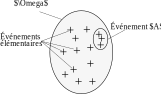
\includegraphics[width=0.6\linewidth]{pics/possibles.pdf}
 
\end{center}
 \caption{Espace des possibles, événements élémentaires et événement $A$}
 \label{fig:possibles}
\end{figure}

On remarquera (voir Fig. \ref{fig:possibles}) que $P(\Omega) = 1$. En effet, il est par définition \emph{certain} que l'issue soit dans $\Omega$.

\section{Opérations sur les événements}

\subsection{Opérations de base}

Soient $A$ et $B$ deux événements et $\omega$ un événement élémentaire. Tous trois appartiennent à l'espace fondamental $\Omega$.

\begin{enumerate}
 \item L'intersection $A \cap B$: $\omega \in A \cap B \Leftrightarrow \omega \in A$ \textbf{et} $\omega \in B$ (fig. \ref{fig:Venn1});
 \item La réunion $A \cup B$: $\omega \in A \cup B \Leftrightarrow \omega \in A$ \textbf{ou} $\omega \in B$. 
 
 $P(A \cup B) = P(A) + P(B) - P(A \cap B)$;
 \item Le complémentaire $\overline{A}$: $\omega \in \overline{A} \Leftrightarrow \omega \nin A$.
\end{enumerate}

\begin{figure}[h!]
\begin{center}
% \begin{tikzpicture}
% \coordinate (A) at ( 90:1.2);
% \coordinate (B) at (250:1.2);
%   \begin{scope}[blend group = soft light]
%     \fill[red!30!white]   (A) circle (2);
%     \fill[green!30!white] (B) circle (2);
%   \end{scope}
%   \node [font=\Large] at (A)   {$A$};
%   \node [font=\Large] at (B)   {$B$};
%   \node [font=\Large, rotate=-10] at (0,0) {$A \cap B$};
% \end{tikzpicture}
    \begin{tikzpicture}
        \begin{scope}[blend group = soft light, rotate=0]
            \draw[] (0,0) ellipse (3 and 2); % E
            \fill[green!30!white] (0,0) ++ (-0.8,0) circle (1); % A
            \fill[red!30!white] (0,0) ++ (0.8,0) circle (1); % B
        \end{scope}
        \node[] (gnieh) at(-2.5,2.0){\Large{$\Omega$}};
        \node[] (A) at(-2.5,-2.5){\Large{$A$}};
        \node[] (B) at(2.5,-2.5){\Large{$B$}};
        \node[] (AinterB) at(0,-2.5){\Large{$A \cap B$}};
        \draw[]  (B) -- (1.8,0);
        \draw[]  (A) -- (-1.8,0);
        \draw[]  (AinterB) -- (0,0);
    \end{tikzpicture}
\end{center}
\caption{Illustration de l'intersection $A \cap B$; $A \cup B$ est la réunion des deux disques.}
\label{fig:Venn1}
\end{figure}

\begin{definition}{événements incompatibles} 
    Deux événements sont \emph{incompatibles} ou \emph{disjoints} lorsqu'ils ne peuvent se réaliser en même temps (fig. \ref{fig:VennIncompat}).    
    On a alors $A \cap B = \emptyset$ soit $P(A \cap B) = 0$.
\end{definition}

Par exemple sur un lancer de dés, \og{}obtenir un nombre plus grand que 4\fg{} et \og{}obtenir un nombre plus petit que 3\fg{} sont des événements incompatibles car ils ne peuvent se réaliser en même temps. 

On a donc: $A \cap B = \emptyset$ et $P(A \cap B) = 0$.

\begin{figure}[h!]
\begin{center}
  \begin{tikzpicture}
  \begin{scope}[blend group = soft light, rotate=0]
      \draw[] (0,0) ellipse (3 and 2); % E
      \fill[green!30!white] (0,0) ++ (-1.2,0) circle (1.0); % A
      \fill[red!30!white] (0,0) ++ (1.2,0) circle (1.0); % B
  \end{scope}
  \node[] (Omega) at(-2.5,2){\Large{$\Omega$}};
  \node[] (A) at(-2.5,-2){\Large{$A$}};
  \node[] (B) at(2.5,-2){\Large{$B$}};
  \draw[]  (B) -- (1.8,0);
  \draw[]  (A) -- (-1.8,0);
\end{tikzpicture}
\end{center}
\caption{Événements disjoints: $A \cap B = \emptyset$}
\label{fig:VennIncompat}
\end{figure}

\subsection{Probabilités conditionnelles}

Soient 2 événements $A$ et $B$ de $\Omega$. 

\begin{definition}{\og{}$A$ sachant $B$\fg{}}
    Soient 2 événements $A$ et $B$ de $\Omega$. 
 On appelle $A$ sachant $B$ (et probabilité de $A$ sachant $B$) la probabilité que l'événement $A$ se produise \emph{sachant que} $B$ est réalisé. 
 Sa probabilité se note $P_B(A)$ et se calcule ainsi: 

 \begin{equation*}
  P_B(A) = \dfrac{P(A\cap B)}{P(B)}
 \end{equation*}
\end{definition}


\subsection{Arbre de probabilité}

Certaines expériences aléatoires peuvent être résumées dans un arbre de probabilités. Pour illustrer cela, nous allons considérer l'expérience suivante:

Une urne contient 5 boules vertes et 3 boules rouges. On en tire deux au hasard sans remise. L'univers des possibles est $\Omega = \{ VV;VR;RV;RR \}$.

Au premier tirage: il y a 5 boules vertes et 3 boules rouges dans l'urne. Pour le premier tirage, on a donc $P(V) = \frac{5}{8} = 0.625$ et $P(R) = \frac{3}{8} = 0.375$.

On remarque que pour le second tirage, les probabilités sont impactées par le résultat du premier tirage:

\begin{itemize}
 \item si on a tiré une boule verte: la probabilité de tirer à nouveau une boule verte est $\frac{4}{7} \approx 0.571$;
 \item si on a tiré une boule rouge: la probabilité de tirer une boule verte est $\frac{5}{7} \approx 0.714$.
\end{itemize}

La situation se résume donc comme on peut le voir figure \ref{fig:arbre}: 

% Set the overall layout of the tree
\tikzstyle{level 1}=[level distance=4.5cm, sibling distance=4cm]
\tikzstyle{level 2}=[level distance=4.5cm, sibling distance=3cm]

% Define styles for bags and leafs
\tikzstyle{bag} = [text width=4em, text centered]
\tikzstyle{end} = [circle, minimum width=3pt,fill, inner sep=0pt]

% The sloped option gives rotated edge labels. Personally
% I find sloped labels a bit difficult to read. Remove the sloped options
% to get horizontal labels. 

\begin{figure}
    \centering
\begin{tikzpicture}[grow=right, sloped]
    \node[bag] {$\Omega$}
    child {
        node[bag] {$R$}        
        child {
            node[end, label=right:
            {$RR$}] {}
            edge from parent
            node[above] {$P_R(RR)$}
            node[below]  {$\frac{2}{7}$}
        }
        child {
            node[end, label=right:
            {$RV$}] {}
            edge from parent
            node[above] {$P_R(RV)$}
            node[below]  {$\frac{5}{7}$}
        }
        edge from parent 
        node[above] {$P(R)$}
        node[below]  {$\frac{3}{8}$}
    }
    child {
        node[bag] {$V$}        
        child {
            node[end, label=right:
            {$VR$}] {}
            edge from parent
            node[above] {$P_V(VR)$}
            node[below]  {$\frac{3}{7}$}
        }
        child {
            node[end, label=right:
            {$VV$}] {}
            edge from parent
            node[above] {$P_V(VV)$}
            node[below]  {$\frac{4}{7}$}
        }
        edge from parent         
        node[above] {$P(V)$}
        node[below]  {$\frac{5}{8}$}
    };
\end{tikzpicture}
\caption{Arbre de probabilités}
\label{fig:arbre}
\end{figure}

L'arbre fig. \ref{fig:arbre} permet de répondre aisément aux questions suivantes:

\begin{enumerate}
 \item Calculer $P(RV)$. 
 
 Pour ce faire, il faut multiplier les probabilités rencontrées dans l'arbre sur le chemin allant de $\Omega$ à $RV$. Ici: $P(RV) = \frac{3}{8} \times \frac{5}{7} = \frac{15}{56} \approx 0.268$;
 \item Calculer la probabilité d'obtenir $V$ au second tirage, indépendamment du résultat du premier tirage.
 
 2 chemins mènent à l'événement \og{}obtenir $V$ au second tirage\fg{}. Il s'agit donc de la somme des probabilités de ces deux chemins: $\frac{5}{8} \times \frac{4}{7} + \frac{3}{8} \times \frac{5}{7} = \frac{35}{56} \approx 0.625$.
\end{enumerate}

\section{Mesure de probabilité, propriétés}

Soient $A$ et $B$ deux événements de l'espace fondamental $\Omega$.

\paragraph{Espace fondamental et ensemble vide}
$P(\Omega) = 1$ et $P(\emptyset) = 0$

\paragraph{Réunion de deux événement quelconques}
$P(A \cup B) = P(A) + P(B) - P(A \cap B)$

\paragraph{Réunion de deux événement disjoints}
Dans ce cas, $P(A \cap B) = 0$. On a donc:

$P(A \cup B) = P(A) + P(B)$

\paragraph{Complémentaire d'un événement}
$P(\overline{A}) = 1 - P(A)$

Exemples:

On donne deux événements $A$ et $B$ incompatibles tel que:  $P(A) =  0.43$ et $P(B) = 0.55$. 

Calculer $P(A \cap B)$, $P(\overline{A})$, $P(\overline{B})$, $P(A \cup B)$ et $P(\overline{A \cup B})$

\cadre{2}

On donne deux événements $A$ et $B$ tels que:  $P(A) =  0.33$, $P(B) = 0.45$ et $P(A \cap B) = 0.21$

Calculer $P(\overline{A})$, $P(\overline{B})$, $P(A \cup B)$, $P(\overline{A \cup B})$ et $P(\overline{A \cap B})$

\cadre{4}


\section{Opérations sur les variables aléatoires}

\subsection{Règles}

Dans ce paragraphe, nous considérerons deux variables aléatoires $X$ et $Y$. et deux nombres $a, b \in \mathbb{R}$. $X$ et $Y$ peuvent être discrètes ou continues, mais pour que les règles opératoires énoncées ici soient valables\footnote{Dans les opérations où $X$ et $Y$ sont mises en jeu, comme $X+Y$, $X-Y$, etc.}, elles doivent être \textbf{indépendantes}. 

Lorsque des variables aléatoires quantitatives sont additionnées/soustraites entre elles ou multipliées par un nombre, cela donne une nouvelle variable aléatoire. On peut par exemple considérer les variables suivantes:

\begin{itemize}
 \item $Z = aX + b$
 \item $S = X + Y$
 \item $D = X - Y$
\end{itemize}

Les espérance, écart-type et variance de $Z$, $S$ et $D$ se calculent comme suit:

\begin{tabular}{|l|l|l|l|}
\hline
                    & $A = aX+b$            & $S=X+Y$                                    & $D=X-Y$                                                                               \\ \hline
\textbf{Espérance}  & $E(A) = aE(X)+b$      & $E(S) = E(X)+E(Y)$                         & $E(D) = E(X)-E(Y)$                                                                    \\ \hline
\textbf{Variance}   & $V(A) = a^2V(X)$      & $V(S)=V(X)+V(Y)$                           & $V(D)=V(X)+V(Y)$                                                                      \\ \hline
\textbf{Écart-type} & $\sigma(A) = |a|V(X)$ & $\sigma(S)=\sqrt{\sigma^2(X)+\sigma^2(Y)}$ & $\sigma(D)=\sqrt{\sigma^2(X)+\sigma^2(Y)}$ \\ \hline
\end{tabular}


\section*{Exercices}

\exo[1]{Entreprise}

Dans une entreprise de 300 salariés, on compte 40\% de femmes et 60\% d'hommes.

De plus 65\% des hommes et 45\% des femmes sont syndiqués.

On choisit au hasard un salarié de l'entreprise; chaque personne a la même probabilité d'être choisie.

On considère les événements:

\begin{itemize}
    \item $H$: \og{}La personne est un homme\fg{};
    \item $F$: \og{}La personne est une femme\fg{};
    \item $S$: \og{}La personne est syndiquée\fg{}
\end{itemize}

\question{}
Représenter l'expérience à l'aide d'un arbre de probabilité

\question{}
Les événements $H$ et $F$ sont-ils incompatibles? Les événements $H$ et $S$ sont-ils incompatibles?

\question{}
Compléter le tableau ci-dessous.

\begin{center}
 \begin{tabular}{|c|c|c|c|}
    \hline
    & $H$ & $F$ & Total \\ \hline
    $S$            &  \hspace{2cm}   &  \hspace{2cm}   &   \hspace{2cm}    \\ \hline
    $\overline{S}$ &     &     &       \\ \hline
    Total          &     &     & 300   \\ \hline
\end{tabular}
\end{center}

\question{}
Déterminer $P(H)$ et $P(F)$.

\question{}
Calculer les probabilités $P(H \cap S)$, $P(F \cap S)$ et $P(S)$.

\question{}
Calculer les probabilités $P(H \cup S)$, $P(F \cup S)$.

\exo[0]{}
Un appareil peut tomber plusieurs fois en panne sur une période déterminée. On note $a_n$ l'événement \og{}l'appareil a eu exactement $n$ pannes\fg{}. Une enquête statistique permet d'admettre les probabilités suivantes:

\begin{center}
\begin{tabular}{|l|l|l|l|l|l|}
    \hline
    $a_n$    & $a_0$ & $a_1$ & $a_2$ & $a_3$ & $a_4$ \\ \hline
    $P(a_n)$ & 0.78  & 0.11  & 0.06  & 0.03  &       \\ \hline
\end{tabular}
\end{center}

\question{}
Sachant qu'il ne peut y avoir plus de 4 pannes, déterminer $P(a_4)$.

\question{}
Quelle est la probabilité qu'un appareil tombe en panne 1 fois? pas plus de 2 fois?

\exo[1]{}
On donne les événements $A$ et $B$ tels que $P(A) = 0.61$ et $P(B) = 0.27$

Calculer $P(A \cup B)$ dans les cas suivants: 

\begin{itemize}
    \item A et B sont incompatibles;
    \item $P(A \cap B) = 0.13$.
\end{itemize}


\exo[3]{}
Un club de vacances propose deux activités nautiques à ses clients: voile ou planche à voile.

Au mois de juillet, le club compte 250 vacanciers.
\begin{itemize}
    \item 30\% font de la planche à voile (P);
    \item 48\% font de la voile (V);
    \item 16\% font les deux activités.
\end{itemize}

$P$ représente l'ensemble des vacanciers qui pratiquent la planche à voile.

$V$ représente l'ensemble des vacanciers qui pratiquent la voile.

On considère les événements suivants: 

\begin{itemize}
    \item A: \og{}Le vacancier choisi pratique au moins une des deux activités\fg{};
    \item B:\og{}Le vacancier choisi ne pratique aucune activité\fg{};
    \item C: \og{}Le vacancier choisi ne pratique qu'une seule activité\fg{}.
\end{itemize}

\question{}
Recopier et compléter le tableau ci-après en indiquant le nombre d'éléments de chaque ensemble.

\begin{center}
    \begin{tabular}{|c|c|c|c|}
        \hline
        & $P$ & $\overline{P}$ & Total \\ \hline
        $V$            &  \hspace{2cm}   &  \hspace{2cm}   &   \hspace{2cm}    \\ \hline
        $\overline{V}$ &     &     &       \\ \hline
        Total          &     &     &    \\ \hline
    \end{tabular}
\end{center}



\question{}
Traduire les événements $A$, $B$ et $C$ en termes d'ensembles ($X \cap Y$, $H \cup Z$...).

\question{}
Calculer $P(A)$, $P(B)$ et $P(C)$.

\exo[3]{Dés}
On jette deux dés équilibrés. Quelle est la probabilité d'obtenir:

\begin{itemize}
 \item un total égal à 7?
 \item un total strictement supérieur à 9?
 \item un total au moins égal à 3?
\end{itemize}


\exo[1]{Cave}
Une personne possède une cave de 2400 bouteilles de vin, rouge et blanc, de trois régions: Bordeaux, Bourgogne et Loire.

La moitié de ses vins sont des Bordeaux, et il y a deux fois plus de bouteilles venant de Bourgogne que de bouteilles venant de Loire.

75\% des vins sont rouges et parmi eux, 54\% viennent du Bordelais. Dans les vins de Loire, il y a autant de blancs que de rouges.

\question{}
Compléter le tableau suivant.

\begin{center}
    \begin{tabular}{|l|l|l|l|l|}
        \hline
        & Bordeaux & Bourgogne & Loire & Total \\ \hline
        Blanc &     \hspace{2cm}     &      \hspace{2cm}     &   \hspace{2cm}    &   \hspace{2cm}    \\ \hline
        Rouge &          &           &       &       \\ \hline
        Total &          &           &       &       \\ \hline
    \end{tabular}
\end{center}


\question{}
On prend au hasard, une bouteille dans cette cave. Calculer la probabilité des événements suivants:

\begin{itemize}
    \item A: \og{}le vin est blanc\fg{};
    \item B: \og{}le vin vient de Bordeaux\fg{}.
\end{itemize}

\question{}
À l'aide d'une phrase, expliciter les événements $A \cap B$ et $A \cup B$ puis calculer leurs probabilités respectives.

\question{}
On choisit une bouteille de vin blanc. Calculer la probabilité que ce soit un Bordeaux

\question{}
On choisit une bouteille de Bourgogne. Calculer la probabilité que ce soit un vin blanc.
%Utiliser le fichier d'à côté pour les exemples (typiquement un grand II ou un grand III)

\end{document}

